% Volume III, Paper 6 (drafted as "Chapter 32")
\chapter{Hecke Algebras on Chambers, Iwasawa Modules, and the \texorpdfstring{$2$}{2}-adic Valuation Tower}\label{chap:V3P6}
\chaptermark{Hecke Algebras and Iwasawa Modules}
\begin{chapterabstract}
The proposed programme asks for three things. (a) The operators of this volume --- $\DeltaH$, $L_E$
and the chiral Kuramoto derivative --- are to be realized in representations of the degenerate
affine Hecke algebra $\mathbb H_d$. (b) A non-commutative $p$-adic $L$-element $L_p(Y)\in
K_1(\Sigma^{-1}\Lambda)$ is to be built from $\det(I-uC^{(d+1)})$, where $\Lambda=\Z_p[[G]]$.
(c) A ``main conjecture'' $\partial L_p(Y)=[\mathrm{Sel}(Y/G)^{\vee}]$ is to be proved by a
five-step scheme. This closing chapter states what is true.

(1) \emph{Hecke algebras.} We give $\mathbb H_d$ and its polynomial representation, checked
exactly. Every operator $L$ is $x_1$ in the $\mathbb H_d$-module $s_i\mapsto1$, $x_i\mapsto
L+(i-1)c$, so ``realized in a representation of $\mathbb H_d$'' has no content. The algebra that
acts naturally is the Iwahori--Hecke algebra $H_q(\Atwo)$ with parameter $q$, acting on
functions on chambers. We prove that the quadratic and braid relations hold on every complex
satisfying (L), including $Y_{21}$, which fails the flag condition. In this language
$\Delta_2=3+T_0+T_1+T_2$, $A_1=(q+1)^{-1}\sum_t\pi_t\pi_{t+1}^{t}$, and
$L_E=(q(q+1))^{-1}\,p\,T_tT_{t+2}T_t\,p^{t}$ blockwise. The vertex operators are images of
symmetric polynomials under the Satake parameters: $A_1=qe_1$, $A_2=qe_2$, $e_3=1$. The
Kuramoto derivative is nonlinear and is not an algebra representation. Its linearization at the
twisted states is $-c_m\Delta_0$, which is central in this sense.

(2) \emph{Localization.} We state Cohn localization and its $K$-theory sequence correctly, and
note that the ``$\to0$'' holds when $K_0(\Lambda)\to K_0(\Sigma^{-1}\Lambda)$ is injective.
Garland rigidity (Chapter~\ref{chap:V3P1}) implies that every open subgroup of a tower group has \emph{finite}
abelianization. So no quotient $G/H\cong\Z_p$ exists, and the Ore set of
Coates--Fukaya--Kato--Sujatha--Venjakob, with its category $\mathfrak M_H(G)$, is \emph{not
available} for any tower over a thick complex. One must localize at all nonzero elements of the
domain $\Lambda$.

(3) \emph{The theorem that replaces the conjecture.} For every infinite pro-$p$ tower, the
equivariant Hecke--Laplacian $\DeltaH_\Lambda\in M_n(\Lambda)$ is injective. If the tower group is
moreover $p$-adic analytic, then $X=\coker\DeltaH_\Lambda$ is a torsion module of projective
dimension $\le1$, and $\mathcal L=[\DeltaH_\Lambda]\in K_1(Q(\Lambda))$ satisfies
$\partial\mathcal L=[X]$. In all cases descent gives $X_U\cong\Z_p\oplus\JacH(Y_U)\otimes\Z_p$. For every
nontrivial Artin representation $\rho$, $\rho(\mathcal L)=\det\DeltaH_\rho\neq0$, and there is
an analytic class number formula
$\prod_{\rho\ne1}\det(\DeltaH_\rho)^{\dim\rho}=[G:U]\,|\JacH(Y_U)|/|\JacH(Y)|$. This formula is
checked exactly on the abelian covers of $X_3$; on $Y_{21}$ the product is $7^{18}$. The
``Selmer group'' has no definition for a complex. Replacing it by $X$ makes $\partial\mathcal
L=[X]$ a theorem, whose content is the descent and the class number formula. Of the five
proposed steps, one is used in a different role, one is not needed, and three do not apply
(Section~\ref{V3P6:sec:five}).

(4) \emph{The canonical tower (Sections~\ref{V3P6:sec:cs}--\ref{V3P6:sec:growth}).} The
triples of the Vol.~I--II presentation satisfy $x+2y+4z\equiv0\pmod7$. So $a_x\mapsto1+\alpha^{x}\varphi$
embeds $\Gamma$ in the cyclic division algebra $(\F_8(t)/\F_2(t),\mathrm{Frob},t)$. The building
is therefore the Bruhat--Tits building of $\PGL_3(\F_2((s)))$, $s=1+t$; it is not exotic. The
closure of $\pi_1(X_3)$ in the units of the maximal order at $t=0$ is a pro-$2$ group $P$ with
$d(P)=3$ and \emph{infinite rank}. This gives an unconditional exhausting pro-$2$ tower, whose
level~$2$ is $Y_{24}$. Its group is \emph{not} $p$-adic analytic: the proposed ``uniform pro-$p$
group with Lie algebra $\mathfrak{pgl}_3$'' does not exist here. $\Gamma$ is discrete in
$\PGL_3(\F_2((s)))$, so no congruence map exists at that place. Along any exhausting tower
$\frac1n\log|\JacH|\to h_H(2)=2.063693$, a Plancherel integral; the tower gives $1.8629$,
$2.0416$, $2.0544$, $2.0625$. The growth of the $2$-part stays open.

(5) \emph{Retrospect and outlook.} We summarize the six chapters of Volume~III, and we list the
open problems that Volume~IV inherits.
\end{chapterabstract}

\section*{Status of the results}

Every numbered statement is proved, apart from the classical inputs, which are marked where
they are used: the PBW theorem and the center of $\mathbb H_d$ \cite{Lus89}, Neumann's theorem
that $\Z_p[[G]]$ is a domain \cite{Neu88}, and the localization sequences \cite{NR04}.
Parts (i$'$) and (ii) of Theorem~\ref{V3P6:thm:main} need a $p$-adic analytic tower
(Hypothesis~(T)); the other parts need only an infinite pro-$p$ tower (T$_p$). Such a tower exists
over $X_3$ for $p=2$ (Theorem~\ref{V3P6:thm:tower}), which answers Chapter~\ref{chap:V3P1},
Remark~\ref{V3P1:rem:scope}(c), for the Vol.~I--II complexes. Further quoted inputs are
Lazard's rank criterion \cite{DDMS}, Oppenheim's trickling-down theorem \cite{Opp18}, Macdonald's
Plancherel measure \cite{Mac71}, and, only in Remark~\ref{V3P6:rem:analytic}, Margulis
\cite{Mar91}. The identities are checked by \texttt{code/v3p6\_verify.py} and
\texttt{code/v3p6\_deep\_verify.py} (Table~\ref{V3P6:tab:battery}).

\section{Hecke algebras}\label{V3P6:sec:hecke}

\begin{definition}[Degenerate affine Hecke algebra \cite{Dri86,Lus89}]\label{V3P6:def:dah}
Let $c\in\C$. $\mathbb H_d$ is generated by $s_1,\dots,s_d$ and $x_1,\dots,x_{d+1}$ subject to
the relations: the $s_i$ satisfy the Coxeter relations of $S_{d+1}$; $x_ix_j=x_jx_i$;
$s_ix_j=x_js_i$ for $j\notin\{i,i+1\}$; and $s_ix_{i+1}-x_is_i=c$. By the PBW theorem,
$\mathbb H_d=\C[S_{d+1}]\otimes\C[x_1,\dots,x_{d+1}]$ as vector spaces. Its center is
$\C[x]^{S_{d+1}}$, and its finite-dimensional irreducible modules have dimension at most
$(d+1)!$ \cite{Lus89}.
\end{definition}

\begin{proposition}[Two representations]\label{V3P6:prop:reps}
\begin{enumerate}
\item[(i)] On $\C[y_1,\dots,y_{d+1}]$, the assignment $x_i\mapsto y_i$ and $s_i\mapsto\sigma_i-c\,\partial_i$,
where $\partial_if=(f-\sigma_if)/(y_i-y_{i+1})$, is a representation.
\item[(ii)] For \emph{every} endomorphism $L$ of a vector space $M$, the assignment
$s_i\mapsto1$, $x_i\mapsto L+(i-1)c$ is a representation on $M$ with $x_1=L$.
\end{enumerate}
In particular, ``$L$ is realized in a representation of $\mathbb H_d$'' holds for every $L$,
and it says nothing about $L$.
\end{proposition}

\begin{proof}
(i) We have $\partial_i\sigma_i=-\partial_i$, $\sigma_i\partial_i=\partial_i$ and $\partial_i^{2}=0$, so
$(\sigma_i-c\partial_i)^{2}=1$. Also $\partial_i(y_{i+1}f)-y_i\partial_if=-f$, which gives the
cross relation. The braid relation is checked on all polynomials of degree $\le4$ in line (Dg).
(ii) The $x_i$ commute, and $x_{i+1}-x_i=c$.
\end{proof}

The algebra that acts naturally is the one-parameter Iwahori--Hecke algebra of the affine Weyl
group of type $\Atwo$ \cite{IM65}, acting on functions on chambers. For $i\in\Z/3$, the
\emph{panel of cotype $i$} of a chamber is its edge that misses type $i$. Define $T_i$ on
$\C^{F}$ by $(T_if)(c)=\sum f(c')$, the sum over chambers $c'\ne c$ with the same cotype-$i$
panel.

\begin{theorem}[Iwahori--Hecke action]\label{V3P6:thm:iwahori}
If $Y$ satisfies \textup{(L)}, then $T_i^{2}=(q-1)T_i+q$ and $T_iT_jT_i=T_jT_iT_j$ for
$i\neq j$. So $\C^{F}$ is a module over $H_q(\Atwo)=\langle T_0,T_1,T_2\rangle$. The flag
condition is not needed.
\end{theorem}

\begin{proof}
Each panel lies in $q+1$ chambers, which gives the quadratic relation. A gallery of type
$(i,j,i)$ or $(j,i,j)$ pivots around the vertex $v$ of $c$ of the third type $k$. By (L), the
chambers containing $v$ are the flags of $\PG(2,q)$. Write $c=(P,\ell)$. A non-stuttering
gallery of type $(i,j,i)$ runs $(P,\ell)\to(P',\ell)\to(P',\ell')\to(P'',\ell')$, and it ends at
a flag opposite to $c$: $P''\notin\ell$ and $P\notin\ell'$. Conversely, each opposite flag is
reached by exactly one such gallery, with $P'=\ell\cap\ell'$. The same holds for $(j,i,j)$. So
both products equal the ``opposite flag'' matrix of the star.
\end{proof}

Let $\pi_t\colon\C^{F}\to\C^{V_t}$ sum over the chambers at a vertex of type $t$. For each
cotype $i$, let $p_i\colon\C^{F}\to\C^{E_i}$ sum over the chambers on an edge of that cotype.

\begin{theorem}[The operators of Volume~III in Hecke language]\label{V3P6:thm:ops}
Assume \textup{(L)}. Then:
\begin{enumerate}
\item[(i)] $\Delta_2=3+T_0+T_1+T_2$, with the type-increasing orientation of chambers;
\item[(ii)] $A_1=\frac1{q+1}\sum_t\pi_t\pi_{t+1}^{t}$, so $\DeltaH=(q^{3}-1)+A_1-qA_2$ and
$\Delta_0=2\kappa-A_1-A_2$;
\item[(iii)] $L_E$ maps $\C^{E_t}$ to $\C^{E_{t+2}}$, and on this block
$L_E=\frac1{q(q+1)}\,p_{t+2}\,T_tT_{t+2}T_t\,p_t^{t}$;
\item[(iv)] on the joint eigenspace with Satake parameters $z$ (where $z_1z_2z_3=1$), $A_1=qe_1(z)$
and $A_2=qe_2(z)$. So $\DeltaH$, $\Delta_0$ and $\det P(u)=\prod_i(1-qx_iu)$ are images of
symmetric polynomials, i.e.\ of central elements of $\mathbb H_2$ or of $H_q$ modulo $e_3-1$.
The Kuramoto field of Chapter~\ref{chap:V3P3} is nonlinear. Its linearization at the twisted states,
$-c_m\Delta_0$, is of this central form.
\end{enumerate}
\end{theorem}

\begin{proof}
(i) All incidences $[t:e]$ are $+1$, and distinct chambers share at most one panel.
(ii) $\pi_t\pi_{t+1}^{t}(v,w)$ counts the chambers containing both $v$ and $w$, which is
$q+1$ for an edge $v\to w$. (iii) An edge $e=x\to y$ has cotype $\tau(y)+1$, and $f=y\to z$ has
cotype $\tau(y)-1$. The product $T_tT_{t+2}T_t$ connects exactly the opposite flags at $y$
(proof of Theorem~\ref{V3P6:thm:iwahori}). For $z\notin x$ there are $q(q+1)$ opposite pairs:
$q+1$ lines through $z$, and $q$ points of $x$ off each such line. For $z\in x$ there are none.
(iv) If $P_a(u)=\prod(1-qz_iu)$, then $a=qe_1(z)$ and $q\bar a=q^{2}e_2(z)$.
\end{proof}

\begin{remark}\label{V3P6:rem:graded}
The degenerate algebra $\mathbb H_d$ is Lusztig's graded version of $H_q$, obtained by
filtering at a central character \cite{Lus89}. It models the representations of $H_q$ near a
given Satake parameter. It does not act on the chain spaces of $Y$, and nothing in this volume
needs it. The spectral data of Chapters~\ref{chap:V3P1}--\ref{chap:V3P4} are central characters, i.e.\ Satake parameters; the
non-central operators ($L_E$, $\Delta_2$) live in $H_q$ and its parabolic modules.
\end{remark}

\section{Localization and the absence of a \texorpdfstring{$\Z_p$}{Zp}-direction}\label{V3P6:sec:loc}

\begin{definition}[Cohn localization \cite{Coh85}]\label{V3P6:def:cohn}
Let $\Sigma$ be a set of maps between finitely generated projective $\Lambda$-modules. A ring
map $\Lambda\to\Sigma^{-1}\Lambda$ is the \emph{Cohn localization} if it makes every
$\sigma\in\Sigma$ invertible and is universal with that property. If $\Lambda\to\Sigma^{-1}\Lambda$
is injective and stably flat (for instance, an Ore localization), there is an exact sequence
\cite{NR04}
\[
K_1(\Lambda)\to K_1(\Sigma^{-1}\Lambda)\xrightarrow{\ \partial\ }K_0(\Lambda,\Sigma)\to
K_0(\Lambda)\to K_0(\Sigma^{-1}\Lambda).
\]
Here $K_0(\Lambda,\Sigma)$ is the $K_0$ of $\Sigma$-torsion modules of projective dimension
$\le1$, and $\partial[\alpha]=[\coker\alpha]$ for injective $\alpha\colon\Lambda^{n}\to\Lambda^{n}$
in $\Sigma$ (this is our sign convention). $\partial$ is surjective when $K_0(\Lambda)\to
K_0(\Sigma^{-1}\Lambda)$ is injective, e.g.\ when $\Lambda$ is local and $\Sigma^{-1}\Lambda$
is a skew field.
\end{definition}

The Ore set of \cite{CFKSV} is
$S=\{s\in\Lambda(G):\Lambda(G)/\Lambda(G)s\text{ is finitely generated over }\Lambda(H)\}$.
It requires a closed normal subgroup $H$ with $G/H\cong\Z_p$, and its torsion category is
$\mathfrak M_H(G)$. The proposed programme's $\Sigma$ (``$M/M[p^{\infty}]$ finite, pseudo-null'') is not
this set.

\begin{theorem}[No $\Z_p$-direction]\label{V3P6:thm:nozp}
Let $Y$ satisfy \textup{(L)} with $q\ge2$. Let $G$ be a profinite group that receives
$\pi_1(Y)$ with dense image, so that its open subgroups $U$ correspond to finite covers $Y_U$.
Then every open $U\le G$ has finite abelianization. In particular no open subgroup of $G$ has a
quotient $\Z_p$, and the Ore set $S$ and the category $\mathfrak M_H(G)$ of \cite{CFKSV} do not
exist for any open subgroup of $G$.
\end{theorem}

\begin{proof}
This is Proposition~\ref{V3P1:prop:fab}(i),(ii). $H_1(Y_U;\Z)$ is finite by Garland rigidity,
and it surjects onto a dense subgroup of $U^{\mathrm{ab}}$.
\end{proof}

So the only natural localization is the Goldie quotient. Under the following hypothesis,
$\Lambda$ is a Noetherian domain \cite{Laz65,Neu88}, and the nonzero elements form an Ore set
with skew field of fractions $Q(\Lambda)$.

\begin{itemize}
\item[(T$_p$)] $\pi_1(Y)\to G$ has dense image, where $G$ is an infinite pro-$p$ group. Put
$\Lambda=\Z_p[[G]]$.
\item[(T)] In addition, $G$ is a torsion-free $p$-adic Lie group. (Such $G$ has dimension $\ge3$
and perfect Lie algebra, by Proposition~\ref{V3P1:prop:fab}(iii).)
\end{itemize}
Section~\ref{V3P6:sec:cs} shows that (T$_2$) holds \emph{unconditionally} over $X_3$, for a
canonical tower. It also shows that this tower does \emph{not} satisfy (T).

\section{The Iwasawa module of Hecke Jacobians}\label{V3P6:sec:main}

Under (T$_p$), choose lifts of the vertices of $Y$ to the tower. Each arc $e\colon v\to w$ of $Y$
acquires a voltage $g_e\in G$. Define $\DeltaH_\Lambda\in M_n(\Lambda)$ by
\[
(\DeltaH_\Lambda)_{vw}=(q^{3}-1)\delta_{vw}+\sum_{e:v\to w}g_e-q\sum_{e:w\to v}g_e^{-1},
\]
and put $X(Y/G)=\coker\DeltaH_\Lambda$. For $U$ open normal, $\Z_p[G/U]\otimes_\Lambda\DeltaH_\Lambda$
is $\DeltaH(Y_U)\otimes\Z_p$, after identifying $\Z_p[G/U]^{n}$ with $\Z_p^{V(Y_U)}$.

\begin{theorem}[Main theorem, replacing the main conjecture]\label{V3P6:thm:main}
Assume \textup{(L)}, $q\ge2$, and \textup{(T$_p$)}. Then \textup{(i)}, \textup{(iii)},
\textup{(iv)} and \textup{(v)} hold. If moreover \textup{(T)} holds, so do \textup{(i$'$)} and
\textup{(ii)}.
\begin{enumerate}
\item[(i)] $\DeltaH_\Lambda$ is injective, and $0\to\Lambda^{n}\to\Lambda^{n}\to X\to0$ is exact.
\item[(i$'$)] $\DeltaH_\Lambda$ is invertible over $Q(\Lambda)$, and $X$ is a finitely generated
torsion $\Lambda$-module of projective dimension $\le1$.
\item[(ii)] $\mathcal L(Y/G):=[\DeltaH_\Lambda]\in K_1(Q(\Lambda))$ satisfies
$\partial\mathcal L(Y/G)=[X(Y/G)]$, and every characteristic element of $X$ differs from
$\mathcal L$ by an element of the image of $K_1(\Lambda)$.
\item[(iii)] Descent: $\Z_p[G/U]\otimes_\Lambda X\cong\Z_p\oplus\bigl(\JacH(Y_U)\otimes\Z_p\bigr)$.
\item[(iv)] Interpolation: for every irreducible representation $\rho\ne1$ of $G/U$,
$\rho(\DeltaH_\Lambda)=\DeltaH_\rho$ and $\det\DeltaH_\rho\neq0$. Moreover
\[
\prod_{\rho\neq1}\det(\DeltaH_\rho)^{\dim\rho}=[G:U]\,\frac{|\JacH(Y_U)|}{|\JacH(Y)|}.
\]
\item[(v)] In the variable $u$: $\det P_{Y_U}(u)=\prod_\rho\det P_\rho(u)^{\dim\rho}$, and the
trivial factor is governed by the derivative identity of Theorem~\ref{V3P1:thm:deriv}.
\end{enumerate}
\end{theorem}

\begin{proof}
(i) Let $x\in\Lambda^{n}$ with $\DeltaH_\Lambda x=0$, and let $x_U$ be its image at level $U$.
Then $\DeltaH(Y_U)x_U=0$, so $x_U$ is constant (Lemma~\ref{V3P1:lem:sector} applied to $Y_U$).
That is, $x_U=c_UN_U\mathbf 1$, where $N_U=\sum_{g\in G/U}g$. Compatibility under $U'\subset U$
gives $c_U=[U:U']c_{U'}$. Since $G$ is infinite pro-$p$, the indices $[U:U']$ are unbounded
powers of $p$, so $c_U=0$ and $x=0$. Only (T$_p$) has been used so far. (i$'$) Under (T),
$\Lambda$ is an Ore domain, and an injective square matrix
stays injective over $Q(\Lambda)$ (clear denominators), hence is invertible. Its cokernel has
rank $0$, and $0\to\Lambda^{n}\to\Lambda^{n}\to X\to0$ is a free resolution. (ii) is the
definition of $\partial$. Two characteristic elements have the same image under $\partial$, so
by exactness they differ by an element of the image of $K_1(\Lambda)$. (iii) Tensor products are
right exact. In the proof of Theorem~\ref{V3P1:thm:deriv}, $\coker\DeltaH(Y_U)\cong\Z\oplus\JacH(Y_U)$.
(iv) Over $\C$, $\DeltaH(Y_U)\cong\bigoplus_\rho(\DeltaH_\rho)^{\oplus\dim\rho}$. The kernel is
$\C\mathbf 1$, in the trivial summand. The other eigenvalues have positive real part by the
sector lemma. The product of the nonzero eigenvalues of $\DeltaH(Y_U)$ is
$n_U|\JacH(Y_U)|$ (proof of Theorem~\ref{V3P1:thm:deriv}), and similarly for $Y$. Divide, using
$n_U/n_Y=[G:U]$. (v) The same decomposition applies to $P(u)$.
\end{proof}

\begin{remark}[Finite abelian check]\label{V3P6:rem:check}
Statement (iv) is a finite-level identity, and it holds for every finite regular cover. For the
abelian covers of $X_3$ it is checked exactly (line (CN)):
$|\JacH(X_3)|=147$, and $\prod_{\chi\ne1}\det\DeltaH_\chi$ equals
$7\cdot3\cdot7^{19}/147=7^{18}$ for $Y_{21}$, $8|\JacH(Y_{24})|/147$ for $Y_{24}$, and
$14|\JacH(Y_{42})|/147$ for $Y_{42}$. On $Y_{21}$ the value $7^{18}$ is also $Q_0(1)$ of
Chapter~\ref{chap:V3P1}: two readings of the same determinant. By Theorem~\ref{V3P6:thm:nozp} no infinite
abelian tower exists. $Y_{21}$ and $Y_{42}$ illustrate (iv) only, while $Y_{24}$ is level~$2$
of the canonical $2$-tower of Section~\ref{V3P6:sec:cs}.
\end{remark}

\begin{remark}[What happened to the Selmer group]\label{V3P6:rem:selmer}
``$\mathrm{Sel}(Y/G)$'' has no definition for a simplicial complex. The natural candidate is the
Iwasawa module $X(Y/G)$ of Hecke Jacobians, with $\Z_p$-coinvariants the $p$-parts of the
$\JacH(Y_U)$. With this choice $\partial\mathcal L=[X]$ holds by construction. The non-formal
content is the descent (iii) and the class number formula (iv), in the spirit of Iwasawa theory
for graphs. Because $G^{\mathrm{ab}}$ is finite, there is no Iwasawa $\mu$--$\lambda$ formula
along a $\Z_p$-direction. The total order $|\JacH(Y_U)|$ grows like $e^{h_Hn_U}$
(Theorem~\ref{V3P6:thm:growth}). The growth of the $p$-part is open
(Remark~\ref{V3P6:rem:twopart}).
\end{remark}

\section{The Cartwright--Steger model and the canonical \texorpdfstring{$2$}{2}-tower}\label{V3P6:sec:cs}

Let $E=\F_8=\F_2(\alpha)$ with $\alpha^{3}=\alpha+1$, and let $\sigma(a)=a^{2}$. Put $K=\F_2(t)$ and
let $D$ be the cyclic algebra $(E(t)/K,\sigma,t)$:
$D=\bigoplus_{j<3}E(t)\varphi^{j}$, $\varphi a=\sigma(a)\varphi$, $\varphi^{3}=t$. It is a division
algebra of degree $3$, because $t$ is not a norm from $E(t)$ ($v_t$ of a norm is divisible by $3$).
Let $\Gamma$ be the group of the triangle presentation of Vol.~I--II,
Construction~\ref{M-X:con:thick}, with generators $a_x$ ($x\in\Z/7$) and relations $a_xa_ya_z=1$
for $(x,y,z)\in T$. It acts simply transitively on the vertices of an $\Atwo$ building $B$, and
$\Gamma^{0}=\pi_1(X_3)$ is its type-preserving subgroup of index $3$.

\begin{theorem}[The Cartwright--Steger model, in the style of \cite{CS98}]\label{V3P6:thm:cs}
\begin{enumerate}
\item[(i)] The assignment $a_x\mapsto u_x:=1+\alpha^{x}\varphi$ defines a homomorphism
$\rho\colon\Gamma\to D^{\times}/K^{\times}$. Indeed $u_xu_yu_z=1+t$ for every $(x,y,z)\in T$.
\item[(ii)] Put $s=1+t$. Then $D\otimes\F_2((s))\cong M_3(\F_2((s)))$. The group $\rho(\Gamma)$
acts on the Bruhat--Tits building $B_s$ of $\PGL_3(\F_2((s)))$, and the $\rho(a_x)v_0$ are the
$7$ neighbours of one type of the base vertex $v_0$.
\item[(iii)] $\rho$ is injective, $\rho(\Gamma)$ acts simply transitively on the vertices of
$B_s$, and $B\cong B_s$. In particular the building of Vol.~I--II is Bruhat--Tits, not exotic,
and $X_3,Y_{21},\dots,Y_{168}$ are quotients of the building of $\PGL_3(\F_2((s)))$.
\end{enumerate}
\end{theorem}

\begin{proof}
(i) For $\beta_i\in E$,
$(1+\beta_1\varphi)(1+\beta_2\varphi)(1+\beta_3\varphi)=1+(\beta_1+\beta_2+\beta_3)\varphi
+(\beta_1\sigma\beta_2+\beta_1\sigma\beta_3+\beta_2\sigma\beta_3)\varphi^{2}
+\beta_1\sigma(\beta_2)\sigma^{2}(\beta_3)\,t$. Take $\beta=(\alpha^{x},\alpha^{y},\alpha^{z})$ with
$(x,y,z)\in T$. The triples of $T$ satisfy $x+2y+4z\equiv0\pmod7$, so the last coefficient is
$1$, and the other two coefficients vanish (line (CS); the $\varphi$-coefficient vanishes
because $\{x,y,z\}$ is a line of $\PG(2,2)=\F_8^{\times}/\F_2^{\times}$).

(ii) At $s$, $E\otimes\F_2((s))=\F_8((s))$ is unramified and $t=1+s$ is a unit. So $t=N(e)$ for
some unit $e\in\F_8[[s]]$. Then $\varphi'=e^{-1}\varphi$ satisfies $\varphi'^{3}=1$, so
$D_s\cong(\F_8((s)),\sigma,1)=\operatorname{End}_{\F_2((s))}(\F_8((s)))$, with $\varphi'$ acting as
Frobenius. Let $v_0$ be the class of the lattice $L_0=\F_8[[s]]$. Since
$(\alpha^{x}\varphi)^{3}=t$, the reduced norm is $\mathrm{Nrd}(u_x)=1+t=s$. Also
$u_x=1+\alpha^{x}e\varphi'$ is integral, so $sL_0\subset u_xL_0\subset L_0$ with
$u_xL_0/sL_0=\operatorname{im}\bar u_x$, where $\bar u_x(y)=y+\beta_xy^{2}$,
$\beta_x=\alpha^{x}\bar e$. Similarly $su_y^{-1}L_0/sL_0=\ker\bar u_y=\{0,\beta_y^{-1}\}$. Line (NB)
checks, for every $\bar e\ne0$, that the seven images are the seven hyperplanes of $\F_8$, that the
seven kernels are the seven lines, and that $\ker\bar u_y\subset\operatorname{im}\bar u_x$ iff
$(x,z,y)\in T$ for some $z$. So the link of $v_0$ in $B_s$ is matched with the link of the base
vertex of $B$, incidence for incidence.

(iii) Define $f\colon B\to B_s$ on vertices by $f(\gamma v)=\rho(\gamma)v_0$. This is well defined
because $\Gamma$ is simply transitive on the vertices of $B$. It is simplicial and equivariant,
and by (ii) it is an isomorphism from each vertex star onto the image star. Hence $f$ is a
covering map. $B_s$ is contractible, and $B$ is connected, so $f$ is an isomorphism. If
$\rho(\gamma)=1$, then $f(\gamma v)=f(v)$, so $\gamma v=v$ and $\gamma=1$.
\end{proof}

At $t=0$ the algebra $D_0=D\otimes\F_2((t))$ is a division algebra, with maximal order
$\mathcal O=\F_8[[\varphi;\sigma]]$ and uniformizer $\varphi$. Put
\[
P=(1+\varphi\mathcal O)\big/\bigl(1+t\F_2[[t]]\bigr),\qquad P_m=\text{image of }1+\varphi^{m}\mathcal O .
\]

\begin{theorem}[The canonical $2$-tower]\label{V3P6:thm:tower}
\begin{enumerate}
\item[(i)] $\rho(\Gamma^{0})\subset P$, and its closure is all of $P$.
\item[(ii)] $\Phi(P)=P_2$, so $d(P)=3$, and $|P/P_m|=2^{3(m-1)-\lfloor(m-1)/3\rfloor}$.
\item[(iii)] $d(P_k)\ge\dim_{\F_2}P_k/P_{2k}\ge2k$. So $P$ has infinite rank, and it is not a
$p$-adic analytic group for any $p$.
\item[(iv)] The groups $U_m=\Gamma^{0}\cap\rho^{-1}(P_m)$ are normal in $\Gamma^{0}$, with
$\Gamma^{0}/U_m\cong P/P_m$ and $\bigcap_mU_m=1$. The covers $Y_m=U_m\backslash B$ satisfy
\textup{(L)}, $Y_1=X_3$, and $Y_2=Y_{24}$.
\end{enumerate}
\end{theorem}

\begin{proof}
(i) Each $u_x\equiv1\bmod\varphi$, and $\mathrm{Nrd}(u_x)=1+t$ is a unit at $t=0$, so
$\rho(\Gamma)\subset\mathcal O^{\times}/\F_2[[t]]^{\times}$ and $\rho(\Gamma^{0})\subset P$. The
Schreier generators $u_0^{s}u_xu_0^{-((s+1)\bmod3)}$ reduce modulo $P_2$ to
$\alpha^{x}+1$ or $\alpha^{x}$, and these span $P/P_2\cong\F_8$ (line (FR)). By the Burnside basis
theorem for pro-$p$ groups and (ii), $\overline{\rho(\Gamma^{0})}=P$.

(ii) The level-$k$ quotient $(1+\varphi^{k}\mathcal O)/(1+\varphi^{k+1}\mathcal O)$ is $\F_8$, via
$1+c\varphi^{k}\mapsto c$. In $P$ the centre removes $\F_2$ when $3\mid k$. We have
$[1+a\varphi^{i},1+b\varphi^{j}]\equiv1+(a\sigma^{i}(b)+b\sigma^{j}(a))\varphi^{i+j}$ and
$(1+a\varphi^{i})^{2}=1+a\sigma^{i}(a)\varphi^{2i}$. For $k\ge2$ these values span the level-$k$
quotient of $P$. This depends only on $k\bmod 6$, and it is checked for $k=2,\dots,13$ in line (FR).
By successive approximation in the complete filtered group, $P_2\subset\Phi(P)$. The reverse
inclusion holds because $P/P_2$ is elementary abelian. The order formula counts $3$ bits per
level, minus one at each level divisible by $3$.

(iii) In characteristic $2$, $(1+x)^{2}=1+x^{2}$, and commutators of elements of $P_k$ lie in
$P_{2k}$. So $\Phi(P_k)\subset P_{2k}$ and $d(P_k)\ge\dim P_k/P_{2k}$. A pro-$p$ group is
$p$-adic analytic iff it has finite rank \cite{DDMS}. An infinite pro-$2$ group is not
$p$-adic analytic for odd $p$, because its open pro-$p$ subgroups would be trivial.

(iv) The $U_m$ are preimages of normal subgroups, and they surject by density. Their
intersection is $\ker\rho\cap\Gamma^{0}=1$ (Theorem~\ref{V3P6:thm:cs}(iii)). Covers are local
isomorphisms, so (L) is inherited. $P/P_2\cong(\Z/2)^{3}$ is the maximal elementary abelian
$2$-quotient of $\Gamma^{0}$, since $\dim H_1(X_3;\F_2)=3$. So $Y_2$ is the unique such cover,
$Y_{24}$, and its Hecke Jacobian agrees (line (L2)).
\end{proof}

\begin{corollary}[Status of the hypotheses]\label{V3P6:cor:status}
Over $X_3$ (and each $Y_m$), (T$_2$) holds unconditionally, with $G=P$. Hence
Theorem~\ref{V3P6:thm:main}(i),(iii),(iv),(v) hold unconditionally along the canonical
$2$-tower. The tower does not satisfy (T). Parts (i$'$) and (ii) remain open for it, because we do
not know whether $\Z_2[[P]]$ is Noetherian or has a skew field of fractions.
\end{corollary}

\begin{remark}[Analytic towers]\label{V3P6:rem:analytic}
$\Gamma$ is a cocompact lattice in $\PGL_3(\F_2((s)))$, a rank-$2$ group over a local field of
characteristic $2$, and it is $S$-arithmetic in $D$. Congruence towers at the other places of
$\F_2(t)$ are again characteristic-$2$ groups of infinite rank. By Margulis' superrigidity and
arithmeticity \cite{Mar91}, one expects every representation of $\Gamma$ over a field of
characteristic $0$ to have finite image (we have not re-checked the precise statement). If so, no
infinite $p$-adic Lie tower exists over $X_3$ for any $p$, and (T) is false for every complex of
Vol.~I--II. The request to make (T) unconditional is therefore answered by
Theorem~\ref{V3P6:thm:tower} and Corollary~\ref{V3P6:cor:status}: the natural tower is pro-$2$
and not analytic, and the theory has to be based on (T$_2$), not on (T).
\end{remark}

\section{Growth of Hecke Jacobians}\label{V3P6:sec:growth}

Let $\nu_q$ be the spectral measure of $A_1$ at a vertex of an $\Atwo$ building of order $q$. It
depends only on $q$, because closed-walk counts do. For the Bruhat--Tits building it is
Macdonald's spherical Plancherel measure \cite{Mac71}: $a=q(z_1+z_2+z_3)$ on
$\{|z_i|=1,\ z_1z_2z_3=1\}$, with density proportional to
$\prod_{i<j}|1-z_j/z_i|^{2}/|1-q^{-1}z_j/z_i|^{2}$.

\begin{theorem}[Exponential growth of the Hecke Jacobian]\label{V3P6:thm:growth}
Let $Y_m$ be an exhausting tower of normal covers of a complex satisfying \textup{(L)} with $q\ge2$,
i.e.\ $U_m$ normal, decreasing, and $\bigcap U_m=1$. Then
\[
\lim_{m\to\infty}\frac{\log|\JacH(Y_m)|}{n_m}=h_H(q):=\int\log|q^{3}-1+a-q\bar a|\,d\nu_q(a).
\]
For $q=2$, $h_H(2)=2.063693$. Along the canonical $2$-tower the values are $1.862909$,
$2.041580$ and $2.054414$ at $m=2,3,4$ (line (J)), and $2.062520$ at $m=5$, where $n=6144$
(exploratory run).
\end{theorem}

\begin{proof}
Normality and $\bigcap U_m=1$ make the injectivity radius tend to infinity. Hence the moments
$\frac1{n_m}\Tr(A_1^{j}A_2^{k})$ converge to those of $\nu_q$, and the empirical measures of the
joint eigenvalues converge weakly. They live on a compact subset of $\C$, where polynomials in
$a$ and $\bar a$ are dense. By Theorem~\ref{V3P1:thm:deriv},
$\log|\JacH(Y_m)|=\sum_{a_i\neq\kappa}\log|\mu_i|-\log n_m$. The only zero of $a\mapsto
q^{3}-1+a-q\bar a$ is $a=\kappa$. Trickling down \cite{Opp18} from the link gap gives a uniform
bound: every nontrivial eigenvalue of the normalized $1$-skeleton walk is at most
$\sqrt q/(q+1-\sqrt q)$. Hence
$\operatorname{Re}\mu_i\ge(q^{3}-1)(\sqrt q-1)^{2}/(q+1-\sqrt q)>0$ for all levels and all
$a_i\ne\kappa$. So $\log|\mu|$ is bounded and continuous on a set carrying all the measures, and
the integrals converge.
\end{proof}

\begin{remark}[The $2$-part]\label{V3P6:rem:twopart}
Along the canonical tower, $v_2|\JacH(Y_m)|=0,18,99,289$ for $m=1,2,3,4$, with $n=3,24,192,768$
($|\JacH(X_3)|=147$ is odd). Per vertex this is $0,0.75,0.52,0.38$; per unit of index it is
$0,2.25,1.55,1.13$. No asymptotic law is proved. $P$ is not analytic, so the growth theorems of
analytic Iwasawa theory do not apply, and ``pseudo-null'' and ``characteristic divisor'' have no
established meaning over $\Z_2[[P]]$. The total order grows like $e^{h_Hn}$
(Theorem~\ref{V3P6:thm:growth}). Whether $v_2$ grows linearly in $n$ is open.
\end{remark}

\section{The five-step scheme}\label{V3P6:sec:five}

\begin{center}
\small
\begin{tabular}{p{0.3\textwidth}p{0.62\textwidth}}
\toprule
proposed step & status\\
\midrule
\textcircled{1} Garland excludes $H^{1}$ poles & True fact (Theorem~\ref{V3P1:thm:garland}), but it plays another role. It makes every $U^{\mathrm{ab}}$ finite and so \emph{removes} the $\Z_p$-direction (Theorem~\ref{V3P6:thm:nozp}). The only degenerate factor of $\mathcal L$ is the trivial representation, which is handled in (iv).\\
\textcircled{2} unitary remainder fixes Euler factors & Not used. The remainder of $L_E$ (Chapter~\ref{chap:V3P4}) lives on edges and does not enter the vertex Jacobians.\\
\textcircled{3} $\Z/3$ chirality cancels odd obstructions & Does not apply. What is true is $\det P(u)\in\Z[u^{3}]$ and $\Tr(\Cthree)^{k}=0$ for $3\nmid k$ (Proposition~\ref{V3P1:prop:grading}). No ``odd obstruction'' is defined.\\
\textcircled{4} spectral rigidity: determinant $=$ Fitting ideal & Does not apply in the stated form. Over commutative $\Z_p[G/U]$, $\mathrm{Fitt}_0(\coker M)=(\det M)$ for square $M$, which is a tautology. Over non-commutative $\Lambda$, Fitting ideals are not defined in general, and $K_1$ replaces them.\\
\textcircled{5} spectrum $=$ class field invariants & Does not apply. No class field theory is involved. What is proved is descent and the class number formula (Theorem~\ref{V3P6:thm:main}(iii),(iv)).\\
\bottomrule
\end{tabular}
\end{center}

\section{Volume~III in retrospect, and Volume~IV}\label{V3P6:sec:retro}

\paragraph{What Volume~III established.} Chapter~\ref{chap:V3P1} proved local Garland rigidity from the link gap
alone, the cubic trace identity with and without the flag condition, and the exact Hecke
pencil. Chapter~\ref{chap:V3P2} showed that no higher simplicial sandpile is abelian, and proved the Hodge
factorization of critical groups and exact avalanche means. Chapter~\ref{chap:V3P3} showed that the gauge
sector of chiral Kuramoto dynamics is a gradient flow, and derived the frustrated ground
states and the block spectra. Chapter~\ref{chap:V3P4} proved the unconditional unitary remainder of the geodesic
edge operator, and its Riemann hypothesis equivalent to Ramanujan. Chapter~\ref{chap:V3P5} showed that chamber
public goods reduce to a pairwise game, and that thickness gives no catalysis. Chapter~\ref{chap:V3P6} described
the Hecke action on chambers, the absence of a $\Z_p$-direction, and the Iwasawa module of Hecke
Jacobians. The recurring lesson is that thick $\Atwo$ complexes are \emph{rigid} (Garland) and
\emph{expanding}, and most proposed higher-order effects either collapse to the $1$-skeleton or
are obstructed by rigidity. The surviving structure is spectral and local: links, Satake
parameters, Hecke operators.

\paragraph{What Volume~IV inherits.} Precise open problems. Problems (a) and (b) of the first
version of this list are now settled as far as stated in Sections~\ref{V3P6:sec:cs}
and~\ref{V3P6:sec:growth}. The complexes of Vol.~I--II are Bruhat--Tits quotients in
characteristic $2$ with an unconditional non-analytic pro-$2$ tower, and $|\JacH|$ grows like
$e^{2.063693\,n}$. What remains of them:
(a) whether $\Z_2[[P]]$ admits a localization in which Theorem~\ref{V3P6:thm:main}(ii) holds
(Section~\ref{V3P6:sec:pro2} proves the finite-level form unconditionally and reduces the question
to whether $\Z_2[[P]]$ is an Ore domain), and the characteristic-$0$ statement of
Remark~\ref{V3P6:rem:analytic};
(b) the growth of $v_2|\JacH(Y_m)|$ along the canonical tower;
(c) the vertex block of $L_E$ and the trace identities for $\Atilde d$, $d\ge3$;
(d) universality, or its failure, for the eigenphases of the unitary remainder;
(e) finite-noise thresholds and genuinely nonlinear chamber games;
(f) chimeras and transverse Hopf bifurcations for the triadic lag.
The first plan for Volume~IV (affine Kac--Moody algebras and cosmology) was replaced by the
authors with topological economics and higher-order games, which continue Chapter~\ref{chap:V3P5}. Nothing
proved here points to cosmology. For the geometric problems above, the natural continuation
remains Kac--Moody buildings and their lattices, where Garland-type rigidity may fail.

% Volume III, Chapter 6 -- addendum: the 2-part of the Hecke Jacobian along the canonical tower
% (open problem (b) of Section~\ref{V3P6:sec:retro}).  Verified by code/v3p6_v2_growth.py.
\section{The $2$-part along the canonical tower}\label{V3P6:sec:twopart}

This section takes up Remark~\ref{V3P6:rem:twopart}. We write $G_m=P/P_m$, $n_m=3|G_m|$,
$N_m=P_m/P_{m+1}$ and $d_m=\log_2|N_m|$, so $d_m=2$ if $3\mid m$ and $d_m=3$ otherwise
(Theorem~\ref{V3P6:thm:tower}(ii)). The vertices of $Y_m$ are the pairs $(g,s)$, $g\in G_m$,
$s\in\Z/3$, and the type-increasing arcs are $(g,s)\to(g\theta_{s,x},s+1)$, $x\in\Z/7$, with
the Schreier generators $\theta_{s,x}=\rho(a_0^{s}a_xa_0^{-(s+1)})$ of the proof of
Theorem~\ref{V3P6:thm:tower}. The group $N_m$ is central in $G_{m+1}$ and elementary abelian
(the commutator and square formulas in that proof land in $P_{m+1}$ and $P_{2m}$), and
$Y_{m+1}\to Y_m$ is a regular cover with group $N_m$. Since $\coker\DeltaH(Y_m)=\Z\oplus\JacH(Y_m)$,
the Smith form of $\DeltaH(Y_m)$ has one zero invariant factor; let $e_m$ be the number of its
\emph{even} nonzero invariant factors, i.e.\ the number of cyclic factors of even order in the
invariant-factor decomposition of $\JacH(Y_m)$, and let $\kappa_m$ be the largest $2$-adic
valuation of an invariant factor. Trivially $e_m\le v_2|\JacH(Y_m)|\le\kappa_me_m$.

\begin{proposition}[Block decomposition of a layer]\label{V3P6:prop:layer}
Fix $m\ge1$ and representatives $\tilde g\in G_{m+1}$ of the cosets of $N_m$. Every arc
$e\colon v\to w$ of $Y_m$, $v=(\bar g,s)$ with label $x$, acquires a voltage $c_e\in N_m$ by
$\tilde g_v\theta_{s,x}=c_e\tilde g_w$. For a character $\chi$ of $N_m$ (all of them are real,
with values $\pm1$) put $A_\chi=\sum_e\chi(c_e)E_{vw}$ and
$D_\chi=7I+A_\chi-2A_\chi^{t}\in M_{n_m}(\Z)$.
\begin{enumerate}
\item[(i)] $D_1=\DeltaH(Y_m)$ and $D_\chi\equiv\DeltaH(Y_m)\pmod2$ for every $\chi$. With
$H=(\chi(c))_{\chi,c}$, which satisfies $HH^{t}=2^{d_m}I$,
\[
(H\otimes I)\,\DeltaH(Y_{m+1})\,(H\otimes I)^{-1}=\bigoplus_{\chi}D_\chi .
\]
The conjugation is defined over $\Z[\tfrac12]$, not over $\Z_2$.
\item[(ii)] $\det D_\chi\ne0$ for $\chi\ne1$, and
\begin{gather*}
|\JacH(Y_{m+1})|=2^{-d_m}\,|\JacH(Y_m)|\prod_{\chi\ne1}|\det D_\chi|,\\
v_2|\JacH(Y_{m+1})|=v_2|\JacH(Y_m)|-d_m+\sum_{\chi\ne1}v_2\det D_\chi .
\end{gather*}
\item[(iii)] Each $D_\chi$, $\chi\ne1$, has exactly $e_m+1$ even invariant factors. Hence
$\sum_{\chi\ne1}v_2\det D_\chi\ge(2^{d_m}-1)(e_m+1)$ and
\[
v_2|\JacH(Y_{m+1})|\ \ge\ v_2|\JacH(Y_m)|-d_m+(2^{d_m}-1)(e_m+1).
\]
\item[(iv)] The maps $a_x\mapsto a_{2x}$ and $a_x\mapsto a_{x+1}$ are automorphisms of $\Gamma$
which extend to the tower. They act on $N_m=\{1+c\varphi^{m}\}$ by $c\mapsto c^{2}$ and
$c\mapsto\alpha^{2^{m}-1}c$, and they permute the nontrivial characters of $N_m$ transitively.
Consequently all $D_\chi$, $\chi\ne1$, have the same invariant factors over $\Z_2$.
\end{enumerate}
\end{proposition}

\begin{proof}
The lifts of $v=(\bar g,s)$ are $(c\tilde g_v,s)$, $c\in N_m$, and since $N_m$ is central the
arc of label $x$ at $c\tilde g_v$ ends at $c\tilde g_v\theta_{s,x}=c\,c_e\tilde g_w$. In the basis
indexed by $(c,v)$, $A_1(Y_{m+1})=\sum_eR(c_e)\otimes E_{vw}$, with $R$ the regular
representation of $N_m$. The characters diagonalize all $R(c)$ at once,
$HR(c)H^{-1}=\operatorname{diag}(\chi(c))$; $H\otimes I$ is real, its inverse is
$2^{-d_m}(H^{t}\otimes I)$, and transposition commutes with this conjugation. This gives the
decomposition of $\DeltaH=7+A_1-2A_1^{t}$, and $D_1=\DeltaH(Y_m)$ because the voltages of the
trivial character are $1$. Between two vertices of $Y_m$ there is at most one arc, so $A_\chi$
has entries $\pm1$ exactly on the arcs, and $D_\chi\equiv\DeltaH(Y_m)$ modulo $2$. Finally
$\det H=\pm2^{d_m2^{d_m-1}}$, so $H$ is not invertible over $\Z_2$. This proves (i).

(ii) The spectrum of $\DeltaH(Y_{m+1})$ is the union of the spectra of the $D_\chi$. Its kernel
is $\C\mathbf 1$ by the sector lemma (Lemma~\ref{V3P1:lem:sector}), and it lies in the trivial
block, so the $D_\chi$, $\chi\ne1$, are nonsingular. The product of the nonzero eigenvalues of
$\DeltaH(Y)$ is $\pm n_Y|\JacH(Y)|$ (proof of Theorem~\ref{V3P1:thm:deriv}; this is the step
used in Theorem~\ref{V3P6:thm:main}(iv)). Dividing the identities for $Y_{m+1}$ and $Y_m$, with
$n_{m+1}/n_m=2^{d_m}$, gives the product formula, and $v_2$ of it gives the valuation identity.
This is the class number formula of Theorem~\ref{V3P6:thm:main}(iv) for the layer
$Y_{m+1}/Y_m$, where it is unconditional (Remark~\ref{V3P6:rem:check}).

(iii) For a nonsingular integer matrix, the number of even invariant factors is its corank over
$\F_2$. By (i) the $\F_2$-corank of $D_\chi$ equals that of $\DeltaH(Y_m)$, which is $e_m+1$
because of the zero invariant factor. Each even invariant factor contributes at least $1$ to
$v_2\det D_\chi$, and there are $2^{d_m}-1$ nontrivial characters.

(iv) The set $T$ is invariant under $x\mapsto2x$ and $x\mapsto x+1$ (line (SY)), so both maps
are automorphisms of $\Gamma$, and they preserve $\Gamma^{0}$. On $D$ the first is induced by the
Frobenius $\sigma$ applied to the coefficients of $\F_8[[\varphi;\sigma]]$, which is a ring
automorphism because $\sigma$ commutes with itself; the second by conjugation with $\alpha^{-1}$,
since $\alpha^{-1}(\alpha^{x}\varphi)\alpha=\alpha^{x-1}\sigma(\alpha)\varphi=\alpha^{x+1}\varphi$.
Both fix the centre and the filtration $1+\varphi^{m}\mathcal O$, so they preserve every
$U_m=\Gamma^{0}\cap\rho^{-1}(P_m)$ and induce type-preserving automorphisms $\psi_m$ of the
$Y_m$ that commute with the projections (checked on the vertex model for $m\le5$ in line (SY)). On
$N_m$: $\sigma(1+c\varphi^{m})=1+c^{2}\varphi^{m}$ and
$\alpha^{-1}(1+c\varphi^{m})\alpha=1+\alpha^{-1}c\,\sigma^{m}(\alpha)\varphi^{m}
=1+\alpha^{2^{m}-1}c\,\varphi^{m}$. If $3\nmid m$, then $2^{m}\not\equiv1\pmod7$, so
$\alpha^{2^{m}-1}$ generates $\F_8^{\times}$, and multiplication by it is transitive on the
nontrivial characters of $\F_8$ (identified with $\F_8^{\times}$ through the trace form). If
$3\mid m$, then $N_m=\F_8/\F_2$, on which $\sigma$ has order $3$ and no nonzero fixed point, so
it permutes the three nontrivial characters cyclically. Now let $\psi$ be one of these
automorphisms of the layer, with $\psi(c\cdot\tilde y)=f(c)\cdot\psi(\tilde y)$ for $c\in N_m$.
Writing $\psi(\tilde g_v)=b_v\tilde g_{\psi v}$ with $b_v\in N_m$, the voltage of the image arc is
$c_{\psi e}=f(c_e)\,b_wb_v^{-1}$. Hence $A_\chi$, after the vertex permutation $\psi$, equals
$B\,A_{\chi\circ f}\,B^{-1}$ with $B=\operatorname{diag}(\chi(b_v))$: the blocks of $\chi$ and
$\chi\circ f$ are conjugate by a signed permutation matrix, which is unimodular, and they have
the same Smith form. The orbits of $f$ on the nontrivial characters are transitive, which proves
(iv). The common valuations are $12$, $64$ and $208$ for the layers $m=2,3,4$ (line (V2)).
\end{proof}

\begin{theorem}[The $2$-part at level $5$]\label{V3P6:thm:v2five}
$v_2|\JacH(Y_5)|=1742$, with $n_5=6144$. The invariant factors of $\DeltaH(Y_5)$ have the
$2$-adic profile of Table~\ref{V3P6:tab:twopart}, with $e_5=546$ even factors and
$\kappa_5=11$.
\end{theorem}

\begin{proof}
Proposition~\ref{V3P6:prop:layer}(ii) for the layer $Y_5\to Y_4$ ($d_4=3$, seven twisted blocks
of size $768$) gives $v_2|\JacH(Y_5)|=289-3+7\cdot208=1742$. The valuations $v_2\det D_\chi$
are computed by $2$-adic elimination modulo $2^{30}$, which never reaches the cap (every block
ends with no zero invariant factor, and $\DeltaH(Y_m)$ with exactly one). The same procedure
recovers $99=18-3+7\cdot12$ for $Y_3\to Y_2$ and $289=99-2+3\cdot64$ for $Y_4\to Y_3$ from the
values of Remark~\ref{V3P6:rem:twopart}, which are themselves obtained by direct elimination
(line (V2)); the exact Smith forms at levels $2$ and $3$ agree with the eliminations (line (SM)),
and the traces $\Tr A_1(Y_{m+1})^{k}$, $k=3,6$, equal the sums of the block traces (line (BL)).
Independently, the direct $2$-adic elimination of the $6144\times6144$ matrix gives $1742$
again, together with the profile of the table (line (FD), about three minutes). The block
decomposition also gives $\frac1{n_5}\log|\JacH(Y_5)|=2.062520$, the value of
Theorem~\ref{V3P6:thm:growth} that was obtained there from the full spectrum (line (TO)).
\end{proof}

The number $e_m$ is an invariant of the group ring $\F_2[G_m]$.

\begin{proposition}[Even invariant factors and the Schur complement]\label{V3P6:prop:schur}
Let $\bar f_s=\sum_{x}\theta_{s,x}^{-1}\in\F_2[G_m]$ and $F_m=1+\bar f_1\bar f_0\bar f_2$, and
let $C_m=\F_2[G_m]/\F_2[G_m]F_m$.
\begin{enumerate}
\item[(i)] $\ker_{\F_2}\bigl(\DeltaH(Y_m)\bmod2\bigr)=\ker(I+A_1)\cong\{v\in\F_2[G_m]:vF_m=0\}$,
and $e_m+1=\dim_{\F_2}C_m$.
\item[(ii)] $F_m$ lies in the augmentation ideal $I$ of $\F_2[G_m]$, the projection
$\F_2[G_{m+1}]\to\F_2[G_m]$ maps $F_{m+1}$ to $F_m$, and
$C_{m+1}/I_{N_m}C_{m+1}\cong C_m$, where $I_{N_m}$ is the augmentation ideal of $\F_2[N_m]$.
\item[(iii)] $e_{m+1}\ge e_m$, and $(e_{m+1}+1)/n_{m+1}\le(e_m+1)/n_m$. Hence the limit
$c_e=\lim_m(e_m+1)/n_m$ exists.
\item[(iv)] For $m=2,\dots,5$: $e_m=6,36,99,546$, $\dim C_m=7,37,100,547$, and
$F_m\in I^{3}\setminus I^{4}$ (the Loewy lengths of $\F_2[G_m]$ are $4,10,16,28$). The resulting
bound $e_m+1\ge\dim\F_2[G_m]/I^{3}=10$ ($m\ge3$) does not grow with $m$.
\end{enumerate}
\end{proposition}

\begin{proof}
(i) Identify $\F_2^{V(Y_m)}=\bigoplus_{s}\F_2[G_m]$ by $v\mapsto(v_s)_s$,
$v_s=\sum_gv(g,s)\,g$. Then $(A_1v)(g,s)=\sum_xv(g\theta_{s,x},s+1)$, i.e.\ $(A_1v)_s=v_{s+1}\bar f_s$
(right multiplication, which commutes with the left action of $G_m$). In characteristic $2$,
$v\in\ker(I+A_1)$ iff $v_s=v_{s+1}\bar f_s$ for all $s$, i.e.\ $v_1=v_2\bar f_1$,
$v_0=v_2\bar f_1\bar f_0$ and $v_2=v_0\bar f_2=v_2\bar f_1\bar f_0\bar f_2$. So $v$ is determined
by $v_2$, and $v_2$ is admissible iff $v_2F_m=0$. The left annihilator of $F_m$ is the kernel of
the right multiplication $R_{F_m}$ on $\F_2[G_m]$, whose dimension equals $\dim\coker R_{F_m}
=\dim C_m$. Finally $\dim\ker_{\F_2}\DeltaH(Y_m)$ is the number of invariant factors divisible
by $2$, which is $e_m+1$ (line (E) computes both sides).

(ii) The augmentation of $F_m$ is $1+7^{3}=344\equiv0$. The projection is a ring map sending
$\theta_{s,x}$ to $\theta_{s,x}$, with kernel $I_{N_m}\F_2[G_{m+1}]$ (a two-sided ideal, $N_m$
being normal). $C_{m+1}$ is a left $\F_2[G_{m+1}]$-module, since left multiplication commutes
with $R_{F_{m+1}}$, and $C_{m+1}/I_{N_m}C_{m+1}=\F_2[G_m]/\F_2[G_m]F_m=C_m$.

(iii) $C_m$ is a quotient of $C_{m+1}$, so $e_{m+1}\ge e_m$. The ring $\F_2[N_m]$ is local with
nilpotent maximal ideal $I_{N_m}$ ($N_m$ is a $2$-group). By Nakayama's lemma, lifts of a basis
of $C_m=C_{m+1}/I_{N_m}C_{m+1}$ generate $C_{m+1}$ over $\F_2[N_m]$, so
$\dim C_{m+1}\le|N_m|\dim C_m$, i.e.\ $(e_{m+1}+1)/n_{m+1}\le(e_m+1)/n_m$. A non-increasing
sequence of nonnegative numbers converges.

(iv) Lines (E) and (AU): $I^{k}$ is computed as $\sum_gI^{k-1}(g-1)$ over three generators of
$G_m$, and $F_m$ is reduced against a basis of $I^{k}$. Since the projections map $I^{k}$ onto
$I^{k}$, the depth of $F_m$ is non-increasing in $m$, so $F_m\notin I^{4}$ for all $m\ge2$.
\end{proof}

\begin{theorem}[Bounds]\label{V3P6:thm:v2bounds}
For $m\ge2$:
\begin{enumerate}
\item[(i)] $e_m\le v_2|\JacH(Y_m)|\le\kappa_me_m$, and
$v_2|\JacH(Y_m)|\le\log_2|\JacH(Y_m)|=(h_H(2)/\log2+o(1))\,n_m$ with $h_H(2)/\log2=2.977$.
\item[(ii)] $\dfrac{v_2|\JacH(Y_{m+1})|}{n_{m+1}}\ \ge\ (1-2^{-d_m})\,\dfrac{e_m+1}{n_m}\ \ge\
\tfrac34\,c_e$.
\item[(iii)] If $c_e>0$, then $v_2|\JacH(Y_m)|$ grows linearly in $n_m$:
\[
\liminf_{m\to\infty}\frac{v_2|\JacH(Y_m)|}{n_m}\ \ge\ \tfrac34\,c_e .
\]
If $v_2|\JacH(Y_m)|=o(n_m)$, then $c_e=0$, that is, $e_m=o(n_m)$. If moreover
$\kappa_m=O(\log n_m)$, then $c_e=0$ implies $v_2|\JacH(Y_m)|=o(n_m\log n_m)$.
\end{enumerate}
\end{theorem}

\begin{proof}
(i) is the definition of $e_m$ and $\kappa_m$, and Theorem~\ref{V3P6:thm:growth}.
(ii) By Proposition~\ref{V3P6:prop:layer}(iii),
$v_2|\JacH(Y_{m+1})|\ge v_2|\JacH(Y_m)|-d_m+(2^{d_m}-1)(e_m+1)$, and
$v_2|\JacH(Y_m)|\ge e_m\ge e_2=6\ge d_m$ by Proposition~\ref{V3P6:prop:schur}(iii). Since
$2^{d_m}-1=(n_{m+1}-n_m)/n_m$, dividing by $n_{m+1}$ gives the first inequality, and
$(e_m+1)/n_m\ge c_e$ for every $m$ gives the second. (iii) follows from (i) and (ii).
\end{proof}

\begin{table}[ht]
\centering\small
\renewcommand{\arraystretch}{1.15}
\resizebox{\textwidth}{!}{%
\begin{tabular}{rrrrcccl}
\toprule
$m$ & $n_m$ & $v_2|\JacH(Y_m)|$ & $e_m$ & $v_2/n_m$ & $e_m/n_m$ & $\kappa_m$ & $2$-adic profile of the invariant factors\\
\midrule
1 & 3 & 0 & 0 & 0 & 0 & 0 & --- ($|\JacH(X_3)|=147$)\\
2 & 24 & 18 & 6 & 0.7500 & 0.2500 & 3 & $2^{3}\colon6$\\
3 & 192 & 99 & 36 & 0.5156 & 0.1875 & 6 & $2^{1}\colon9,\ 2^{2}\colon9,\ 2^{3}\colon12,\ 2^{6}\colon6$\\
4 & 768 & 289 & 99 & 0.3763 & 0.1289 & 8 & $2^{1}\colon24,\ 2^{2}\colon23,\ 2^{3}\colon25,\ 2^{4}\colon9,\ 2^{5}\colon12,\ 2^{8}\colon6$\\
5 & 6144 & 1742 & 546 & 0.2835 & 0.0889 & 11 & $2^{1}\colon132,\ 2^{2}\colon83,\ 2^{3}\colon111,\ 2^{4}\colon104,\ 2^{5}\colon64,$\\
  &      &      &     &        &        &    & $2^{6}\colon25,\ 2^{7}\colon9,\ 2^{8}\colon12,\ 2^{11}\colon6$\\
\bottomrule
\end{tabular}}
\caption{The $2$-part of the Hecke Jacobian along the canonical tower. ``$2^{k}\colon c$'' means
$c$ invariant factors of $2$-adic valuation exactly $k$. Lines (SM), (V2), (E), (FD), (TB) of
\texttt{code/v3p6\_v2\_growth.py}.}\label{V3P6:tab:twopart}
\end{table}

\begin{remark}[The data, and what they support]\label{V3P6:rem:v2verdict}
Table~\ref{V3P6:tab:twopart} and line (GR) give the following.
\begin{enumerate}
\item[(a)] $v_2/n_m=0.7500$, $0.5156$, $0.3763$, $0.2835$ for $m=2,\dots,5$, decreasing at
every level. The ratios $v_2(m)/v_2(m-1)$ are $5.500$, $2.919$, $6.028$ against the indices
$8$, $4$, $8$, i.e.\ the local exponents $\log(v_2\text{ ratio})/\log(\text{index})$ are
$0.820$, $0.773$, $0.864$, and the least-squares fit $v_2\sim cn^{\beta}$ over $m=2,\dots,5$
gives $\beta=0.822$ ($0.830$ over $m=3,\dots,5$). Per unit of index, $v_2/(n_m/3)=2.250$,
$1.547$, $1.129$, $0.851$.
\item[(b)] $(e_m+1)/n_m=0.2917$, $0.1927$, $0.1302$, $0.0890$, non-increasing as
Proposition~\ref{V3P6:prop:schur}(iii) requires, with successive ratios $0.661$, $0.676$,
$0.684$. The lower bound of Theorem~\ref{V3P6:thm:v2bounds}(ii) is $0.2552$, $0.1445$, $0.1139$
at $m=3,4,5$, against the actual $0.5156$, $0.3763$, $0.2835$; the layer sums
$\sum_{\chi\ne1}v_2\det D_\chi=84$, $192$, $1456$ exceed the bounds $(2^{d_m}-1)(e_m+1)=49$,
$111$, $700$ by the factors $1.71$, $1.73$, $2.08$.
\item[(c)] At every computed level the largest exponent is $\kappa_m=\log_2|G_m|=\log_2(n_m/3)$
($3,6,8,11$), attained by exactly six invariant factors: the $2$-part of $\JacH(Y_m)$ has
exponent $|G_m|$ and contains $(\Z/|G_m|)^{6}$. We have no explanation. The invariant factors of
the twisted blocks (largest exponent $5$ at the layer $Y_5\to Y_4$) are not those of
$\DeltaH(Y_5)$, as Proposition~\ref{V3P6:prop:layer}(i) warns.
\end{enumerate}
\emph{Verdict.} The conjecture that $\lim v_2|\JacH(Y_m)|/n_m$ exists and is positive is
\emph{not supported by the data}: on the five computed levels the ratio decreases monotonically
from $0.75$ to $0.28$, every local exponent is below $1$, and $(e_m+1)/n_m$ decays geometrically
by a factor of about $0.68$ per level. The data support \emph{sublinear} growth,
$v_2|\JacH(Y_m)|\asymp n_m^{\beta}$ with $\beta\approx0.82$, and, through
Theorem~\ref{V3P6:thm:v2bounds}(iii), they suggest $c_e=0$. This is a statement about five
levels only; the levels $6$--$8$ of Theorem~\ref{V3P6:thm:v2eight} and
Remark~\ref{V3P6:rem:v2eight} weaken it (the decay rates are slowing down), and
Theorem~\ref{V3P6:thm:v2sharp} improves the constant $\frac34$ below to $1$. We have no proof of an asymptotic law in either direction. What is proved is
Theorem~\ref{V3P6:thm:v2bounds}: linear growth follows from $c_e>0$, sublinear growth forces
$c_e=0$, and $c_e$ is the limit of the normalized kernel dimensions of the single element $F_m$
of $\F_2[G_m]$, a mod-$2$ analogue of a von Neumann dimension along the tower, whose
vanishing is the real open question. The augmentation filtration does not decide it: $F_m$ has
depth exactly $3$ for all computed $m$, which gives only $e_m+1\ge10$. Because $P$ has infinite
rank (Theorem~\ref{V3P6:thm:tower}(iii)), $\F_2[[P]]$ is not known to be Noetherian, and the
growth bounds for torsion modules over the Iwasawa algebras of $p$-adic analytic groups are not
available. Open problem (b) of Section~\ref{V3P6:sec:retro} is therefore sharpened to: decide
whether
\[
c_e=\lim_{m\to\infty}\frac{\dim_{\F_2}\bigl(\F_2[G_m]/\F_2[G_m]F_m\bigr)}{n_m}
\]
vanishes.
\end{remark}

\subsection*{Induced characters and levels $6$--$8$}

The layer decomposition of Proposition~\ref{V3P6:prop:layer} uses the central subgroup $N_m$, so
each new level costs $2^{d_m}-1$ blocks of the size of the previous level. Going down to
$Y_k$ with $k\approx m/2$ is much cheaper, because the whole kernel $P_k/P_m$ is still abelian.

\begin{proposition}[Induced characters of $P_k/P_m$]\label{V3P6:prop:induced}
Let $2\le k<m\le2k$ and $A=P_k/P_m\subset G_m$.
\begin{enumerate}
\item[(i)] $A$ is an elementary abelian normal $2$-subgroup, and the coefficients of
$\varphi^{k},\dots,\varphi^{m-1}$ (without the $\F_2$-part of the coefficients of $\varphi^{3i}$)
identify it with $\F_2^{d}$, $2^{d}=n_m/n_k$. The left action of $A$ on $Y_m$ is free, and
$A\backslash Y_m=Y_k$.
\item[(ii)] With coset representatives $r_c\in G_m$ ($c\in G_k$), every arc $c\to c'$ of $Y_k$ with
label $x$ has the voltage $a_e=r_c\theta_{s,x}r_{c'}^{-1}\in A$. For $\chi\in\widehat A$ put
$A_\chi=\sum_e\chi(a_e)E_{cc'}$ and $D_\chi=7I+A_\chi-2A_\chi^{t}$. Then
$\DeltaH(Y_m)$ is conjugate over $\Z[\frac12]$ to $\bigoplus_\chi D_\chi$, $D_1=\DeltaH(Y_k)$,
$D_\chi\equiv\DeltaH(Y_k)\pmod2$, and
\[
v_2|\JacH(Y_m)|=v_2|\JacH(Y_k)|-\log_2\frac{n_m}{n_k}+\sum_{\chi\ne1}v_2\det D_\chi .
\]
\item[(iii)] (Artin--Clifford.) $D_\chi$ is the Hecke operator of $Y_k$ twisted by
$\operatorname{Ind}_A^{G_m}\chi$. $G_m$ acts on $\widehat A$ by conjugation; blocks in one orbit
$O$ are conjugate by signed permutation matrices, hence have the same Smith form over $\Z_2$, and
\[
\prod_{\chi\in O}\det D_\chi=\prod_{\rho\in\operatorname{Irr}(G_m)\text{ over }O}\det\bigl(\Delta^{H}_\rho\bigr)^{\dim\rho}.
\]
\end{enumerate}
\end{proposition}

\begin{proof}
(i) $A$ is the kernel of the projection $G_m\to G_k$, hence normal. For $x,y\in\varphi^{k}\mathcal O$,
$(1+x)(1+y)=1+x+y+xy$ and $xy\in\varphi^{2k}\mathcal O\subseteq\varphi^{m}\mathcal O$, so $A$ is
abelian, the multiplication is addition of coefficients, and every element has order $2$. The
central units $1+t^{i}$ used to normalize only change the $\F_2$-part of the coefficient of
$\varphi^{3i}$, and they also act additively, since the cross terms again lie in
$\varphi^{2k}\mathcal O$. The deck group $G_m$ acts on $Y_m$ by left multiplication and the arcs
are right multiplications, so the left action of any subgroup is free and commutes with the arcs.
(ii) The arc of label $x$ at $ar_c$ ends at $ar_c\theta_{s,x}=(aa_e)r_{c'}$. In the basis
$(a,c)$, $A_1(Y_m)=\sum_eR(a_e)\otimes E_{cc'}$, and the proof of
Proposition~\ref{V3P6:prop:layer}(i)--(ii) applies word for word with $A$ in place of $N_m$; it
never used that $N_m$ is central, only that it is abelian and acts on the left. (iii)
$\C[G_m]=\operatorname{Ind}_A^{G_m}\C[A]=\bigoplus_\chi\operatorname{Ind}_A^{G_m}\chi$, and the
$\chi$-summand is the $\chi$-isotypic part for the left $A$-action, on which $\DeltaH$ acts as
$D_\chi$. For $g\in G_m$, left multiplication by $g$ maps $ar_c$ to $(gag^{-1})(gr_c)$ and
$gr_c=b_cr_{\bar gc}$ with $b_c\in A$; it carries the $\chi$-isotypic part to the
$\chi\circ\operatorname{Ad}(g)^{-1}$-isotypic part, and in the bases above it is the
permutation $c\mapsto\bar gc$ times the signs $\chi(b_c)$. By Clifford's theorem every
irreducible $\rho$ of $G_m$ lies over exactly one orbit, and
$\bigoplus_{\chi\in O}\operatorname{Ind}\chi=\bigoplus_{\rho\text{ over }O}\rho^{\dim\rho}$ as
summands of the regular representation; take determinants of $\DeltaH$ on both sides.
\end{proof}

\begin{theorem}[Levels $6$, $7$, $8$]\label{V3P6:thm:v2eight}
The $2$-parts and the total orders of the Hecke Jacobians of $Y_5,\dots,Y_8$ are:
\begin{center}\small
\begin{tabular}{rrrcc}
\toprule
$m$ & $n_m$ & $v_2|\JacH(Y_m)|$ & $v_2/n_m$ & $\frac1{n_m}\log|\JacH(Y_m)|$\\
\midrule
$5$ & $6144$ & $1742$ & $0.28353$ & $2.062520$\\
$6$ & $49152$ & $11595$ & $0.23590$ & $2.063511$\\
$7$ & $196608$ & $36937$ & $0.18787$ & $2.063639$\\
$8$ & $1572864$ & $254662$ & $0.16191$ & $2.063684$\\
\bottomrule
\end{tabular}
\end{center}
\end{theorem}

\begin{proof}
Proposition~\ref{V3P6:prop:induced} with $(m,k)=(6,3)$: $255$ blocks of size $192$ in $24$
conjugation orbits; $(6,4)$: $63$ blocks of size $768$ in $21$ orbits; $(7,4)$: $255$ blocks in $24$
orbits; $(8,4)$: $2047$ blocks of size $768$ in $52$ orbits (sizes $1^{7},4^{14},64^{31}$). The
block valuations are computed by the $2$-adic elimination of Theorem~\ref{V3P6:thm:v2five} (cap
$2^{30}$, never reached), on one representative of each orbit, and checked to be constant on the
orbit (all members for $m\le6$, two further members of every orbit for $m=7,8$). The two routes to
level $6$ give $99+7-15+11504=289+9-15+11312=11595$, and the two routes to level $7$, over
$Y_4$ and over $Y_5$ ($(m,k)=(7,5)$: $31$ blocks of size $6144$ in $10$ orbits, valuations $1408$
and $1056$), give $289+9-17+36656=1742+12-17+35200=36937$. The same procedure recovers $99$, $289$
and $1742$ from $Y_2$ and $Y_3$, i.e.\ Theorem~\ref{V3P6:thm:v2five} by a route independent of the
central layers. The total orders are the sums of $\log|\det D_\chi|$ (floating point).
\end{proof}

The column of total orders converges to $h_H=2.063693$ from below, the last value being
$9\cdot10^{-6}$ short: the Plancherel limit of Theorem~\ref{V3P6:thm:growth} is visible to five
digits at $n=1.57\cdot10^{6}$. The $2$-part does not converge at that rate, if at all.

\begin{theorem}[A sharper lower bound]\label{V3P6:thm:v2sharp}
For $2\le k<m\le2k$,
\[
v_2|\JacH(Y_m)|\ \ge\ v_2|\JacH(Y_k)|-\log_2\frac{n_m}{n_k}+\Bigl(\frac{n_m}{n_k}-1\Bigr)(e_k+1).
\]
Consequently $\liminf_m v_2|\JacH(Y_m)|/n_m\ge c_e$, improving the constant $\frac34$ of
Theorem~\ref{V3P6:thm:v2bounds}(iii) to $1$. Moreover $e_6=3169$, so
$c_e\le(e_6+1)/n_6=0.06449$.
\end{theorem}

\begin{proof}
By Proposition~\ref{V3P6:prop:induced}(ii) each of the $n_m/n_k-1$ nontrivial blocks is congruent
to $\DeltaH(Y_k)$ modulo $2$, hence has $\F_2$-corank $e_k+1$ and $v_2\det D_\chi\ge e_k+1$ (as in
Proposition~\ref{V3P6:prop:layer}(iii)). For the limit take $k=\lceil m/2\rceil$: then
$n_m/n_k\to\infty$, $\log_2(n_m/n_k)=O(m)=o(n_m)$, $v_2|\JacH(Y_k)|\ge0$, and
$(e_k+1)/n_k\ge c_e$ by Proposition~\ref{V3P6:prop:schur}(iii). The value of $e_6$ is
$\dim\F_2[G_6]/\F_2[G_6]F_6-1$ by Proposition~\ref{V3P6:prop:schur}(i), computed by Gaussian
elimination over $\F_2$ on the $16384\times16384$ matrix of right multiplication by $F_6$
($|\operatorname{supp}F_6|=154$).
\end{proof}

\begin{figure}[t]
\centering
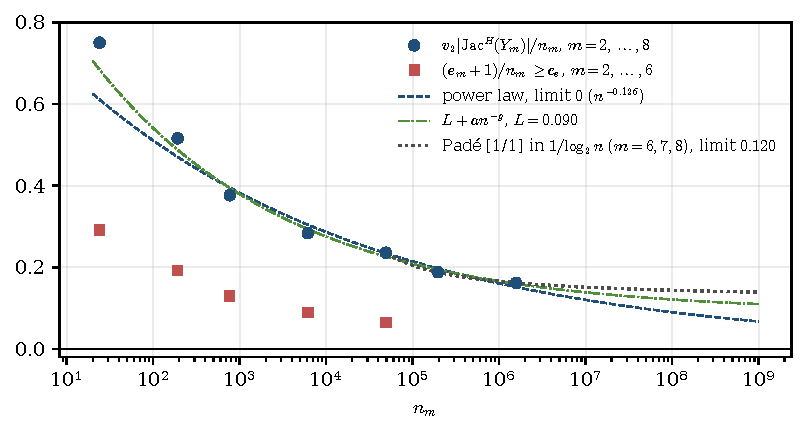
\includegraphics[width=\textwidth]{figures/fig_v2_growth.pdf}
\caption{The $2$-part of the Hecke Jacobian along the canonical $2$-tower: $v_2|\JacH(Y_m)|/n_m$ for
$m=2,\dots,8$ (Theorems~\ref{V3P6:thm:v2five}, \ref{V3P6:thm:v2eight}) and the normalized
$\F_2$-kernel dimensions $(e_m+1)/n_m$ for $m=2,\dots,6$, which decrease to the limit $c_e$
(Proposition~\ref{V3P6:prop:schur}, Theorem~\ref{V3P6:thm:v2sharp}). Three extrapolations of
$v_2/n_m$ that fit the data about equally well: a power law $n^{-0.126}$ with limit $0$ (fitted on
$m=3,\dots,8$); the least-squares optimum $0.090+an^{-g}$ of Remark~\ref{V3P6:rem:v2eight}(b); and the
Pad\'e approximant $[1/1]$ in $1/\log_2n$ through $m=6,7,8$, with limit $0.120$, drawn only on the range
of its data and beyond. The data do not decide between a positive limit and slow decay to $0$; what is
proved is $\liminf v_2/n_m\ge c_e$. Data of \texttt{code/v3p6\_level5\_v2.py}, drawn by
\texttt{code/make\_figures.py}.}
\label{V3P6:fig:v2growth}
\end{figure}

\begin{remark}[The data at levels $2$--$8$]\label{V3P6:rem:v2eight}
The numbers below are produced by lines (FT) and (E) of the script
\texttt{code/v3p6\_level5\_v2.py}.
\begin{enumerate}
\item[(a)] The sequences, with the local exponent
$\beta_m=\log\bigl(v_2(m)/v_2(m-1)\bigr)/\log(n_m/n_{m-1})$ and the ratio
$\rho_m=\bigl((e_m+1)/n_m\bigr)/\bigl((e_{m-1}+1)/n_{m-1}\bigr)$:
\begin{center}\small
\begin{tabular}{lccccccc}
\toprule
$m$ & $2$ & $3$ & $4$ & $5$ & $6$ & $7$ & $8$\\
\midrule
$n_m/n_{m-1}$ & --- & $8$ & $4$ & $8$ & $8$ & $4$ & $8$\\
$v_2/n_m$ & $0.750$ & $0.516$ & $0.376$ & $0.284$ & $0.236$ & $0.188$ & $0.162$\\
$\beta_m$ & --- & $0.820$ & $0.773$ & $0.864$ & $0.912$ & $0.836$ & $0.928$\\
$(e_m+1)/n_m$ & $0.292$ & $0.193$ & $0.130$ & $0.089$ & $0.064$ & & \\
$\rho_m$ & --- & $0.661$ & $0.676$ & $0.684$ & $0.724$ & & \\
\bottomrule
\end{tabular}
\end{center}
$v_2/n_m$ still decreases at every level, and every $\beta_m$ is below $1$. But the exponents are
increasing; along the layers of index $8$ they are $0.820$, $0.864$, $0.912$, $0.928$. Likewise
$(e_m+1)/n_m$ decreases with increasing ratios $\rho_m$, so the geometric decay by a constant factor
suggested by Remark~\ref{V3P6:rem:v2verdict}(b) is not borne out (Figure~\ref{V3P6:fig:v2growth}).
\item[(b)] \emph{Fits.} With limit $L=0$ the best power law is $v_2\sim n^{0.874}$. The
three-parameter model $v_2/n=L+an^{-g}$ fitted on $m=3,\dots,8$ has its least-squares optimum at
$L=0.090$, but the residual at $L=0$ is only $1.09$ times the optimum, and the leave-one-out optima
range over $[0,0.125]$. Exact fits through three consecutive levels jump with the period-$3$
pattern of the indices ($8,4,8,8,4,8$) and are not used. The data do not distinguish a positive
limit of order $0.1$ from slow decay to $0$.
\item[(c)] \emph{Rigorous interval.} $c_e\le\liminf v_2/n_m\le\limsup v_2/n_m\le h_H/\log2=2.977$,
with $0\le c_e\le0.0645$. The bound of Theorem~\ref{V3P6:thm:v2sharp} is far from sharp at finite
level: over $Y_4$ it gives $v_2/n_m\ge0.134,0.131,0.130$ for $m=6,7,8$, against the actual
$0.236,0.188,0.162$.
\item[(d)] \emph{The ratio to $c_e$.} At $m=2k$ the observed quotient
$\bigl(v_2|\JacH(Y_{2k})|/n_{2k}\bigr)\big/\bigl((e_k+1)/n_k\bigr)$ is $1.290,1.224,1.243$ for
$k=2,3,4$: on average a twisted block has about $1.25$ times the minimal valuation $e_k+1$. If this
quotient stays bounded, which would follow from a uniform bound on the $2$-exponents of the blocks
(they are at most $10$ at levels $6$--$8$), then $v_2|\JacH(Y_m)|/n_m$ and $(e_{\lceil m/2\rceil}+1)/n_{\lceil m/2\rceil}$ have the same
order, and $\lim v_2/n_m>0$ iff $c_e>0$.
\end{enumerate}
\emph{Verdict.} Strict positivity of the slope is not decided by levels $2$--$8$. What is proved is
that a positive mod-$2$ kernel density $c_e$ forces slope at least $c_e$; the numbers agree with
slope $\asymp c_e$, and both sequences are still decreasing, but more slowly at every level.
The open problem remains whether $c_e=\lim\dim_{\F_2}(\F_2[G_m]/\F_2[G_m]F_m)/n_m$ vanishes.
\end{remark}

\begin{remark}[Verification]\label{V3P6:rem:v2code}
The script \texttt{code/v3p6\_v2\_growth.py} uses numpy and the sparse module of scipy. It runs
in about five minutes (one minute with \texttt{--quick}, which skips line (FD)). It builds
levels $2$--$5$ (line (LV)), checks
the central elementary abelian layers and the voltages, the trace identities and the Hadamard
decomposition (BL), the valuation identity at the layers $2\to3$, $3\to4$ against the direct
values and its application at $4\to5$ (V2), the agreement of the $2$-adic eliminations with the
exact Smith forms at levels $2,3$ (SM), $e_m$ from the $\F_2$-rank of $I+A_1$ and from
$\dim C_m$ (E), the depth of $F_m$ (AU), the two automorphisms and their action on the
characters (SY), the total order and $v_2\le\log_2|\JacH|$ (TO), the direct elimination of the
$6144\times6144$ matrix (FD), and the table and growth statistics (TB), (GR).

The script \texttt{code/v3p6\_level5\_v2.py} (numpy, matplotlib; about three minutes, plus about
$70$ minutes with \texttt{--check7}) verifies Proposition~\ref{V3P6:prop:induced} and
Theorems~\ref{V3P6:thm:v2eight}, \ref{V3P6:thm:v2sharp}: the quotient models and the
elementary abelian structure of $P_k/P_m$ (QT), the conjugation orbits on the characters (CJ), the
re-derivation of $18,99,289$ by direct elimination and of $99,289,1742$ through induced characters
(VA), the new levels with the two routes to level $6$ (and, with \texttt{--check7}, the route to
level $7$ over $Y_5$) (NW), $e_m+1$ for $m\le6$ and the sharpened bound (E), the total orders (TO),
and the fits (FT). Data and the figure are written to \texttt{data/}.
\end{remark}

% Volume III, Chapter 6 -- addendum: localization over the non-analytic group ring Z_2[[P]]
% (open problem (a) of Section~\ref{V3P6:sec:retro}).  Verified by code/v3p6_pro2_localization.py
% and, for the 2-adic orders, code/v3p6_level5_v2.py.
\section{Localization over the non-analytic group \texorpdfstring{$\Z_2[[P]]$}{Z2[[P]]}}\label{V3P6:sec:pro2}

Corollary~\ref{V3P6:cor:status} leaves parts (i$'$) and (ii) of Theorem~\ref{V3P6:thm:main} open
for the canonical tower, because nothing is known about $\Lambda=\Z_2[[P]]$ beyond what holds for
every pro-$2$ group. This section separates what can be proved about $\Lambda$ from what cannot,
and proves an unconditional substitute for (ii): a compatible system of characteristic elements
at the finite levels, whose boundaries are the finite parts of the Iwasawa module and whose
reduced norms are the Artin factors of the class number formula. Throughout, $G_m=P/P_m$,
$n_m=3|G_m|$, $N_m=\sum_{g\in G_m}g\in\Z_2[G_m]$, and $\DeltaH_\Lambda\in M_3(\Lambda)$ is the
equivariant operator of Section~\ref{V3P6:sec:main} for the tower $Y_m\to X_3$, so that
$\Z_2[G_m]\otimes_\Lambda\DeltaH_\Lambda=\DeltaH(Y_m)\otimes\Z_2$ under
$\Z_2[G_m]^{3}=\Z_2^{V(Y_m)}$.

\subsection*{What is known about \texorpdfstring{$\Lambda$}{Lambda}}

\begin{proposition}[The group $P$ and its ring]\label{V3P6:prop:pro2basic}
\begin{enumerate}
\item[(i)] $P$ is a torsion-free pro-$2$ group, topologically generated by $3$ elements, of
infinite rank; $d(P_k)\ge2k$.
\item[(ii)] $\Lambda=\varprojlim_m\Z_2[G_m]$ is a compact local ring with maximal ideal
$(2,I_P)$, $I_P$ the augmentation ideal, and every finitely generated compact
$\Lambda$-module $M$ satisfies $M=\varprojlim_m\Z_2[G_m]\otimes_\Lambda M$.
\item[(iii)] The necessary condition for $\Lambda$ to be a domain holds: $\Z_2[[P]]$ has no
zero divisor of the form $(g-1)\nu$ with $g$ of finite order and $\nu$ its norm element.
\end{enumerate}
\end{proposition}

\begin{proof}
(i) Generation, rank and $d(P_k)$ are Theorem~\ref{V3P6:thm:tower}. A pro-$2$ group has no
torsion of odd order, so let $x\in1+\varphi\mathcal O$ with $x^{2^{k}}\in K^{\times}$,
$K=\F_2((t))$ the centre of $D_0$. The field $K(x)\subseteq D_0$ has degree $1$ or $3$ over $K$,
since $D_0$ is a division algebra of degree $3$. Over $K(x)$, in characteristic $2$, $y^{2^{k}}-x^{2^{k}}=(y-x)^{2^{k}}$, and the minimal
polynomial $f$ of $x$ over $K$ divides it, so $f=(y-x)^{j}$ with $j=[K(x):K]\in\{1,3\}$. If $j=3$,
then $f=y^{3}+xy^{2}+x^{2}y+x^{3}$ has its coefficients in $K$, so $x\in K$, a contradiction.
Hence $j=1$, $x\in K^{\times}\cap(1+\varphi\mathcal O)=1+t\F_2[[t]]$, and $x$ is
trivial in $P$. (ii) is standard for pro-$p$ groups: $\Lambda/(2,I_P)=\F_2$, and every element
outside $(2,I_P)$ is a unit, being a unit in every $\Z_2[G_m]$, which is local because $G_m$ is
a $2$-group; the limit statement holds because $M$ is a quotient of $\Lambda^{r}$ and inverse
limits of compact modules are exact. (iii) If $g$ has order $p$, then
$(g-1)(1+g+\dots+g^{p-1})=0$; by (i) there is no such $g\ne1$.
\end{proof}

The ring-theoretic questions that (i$'$) and (ii) need are open for $\Lambda$.

\begin{remark}[What is not known]\label{V3P6:rem:pro2open}
\begin{enumerate}
\item[(a)] \emph{Domain.} Neumann's theorem \cite{Neu88} says that $\Z_p[[G]]$ is a domain when
$G$ is a torsion-free \emph{$p$-adic analytic} pro-$p$ group; its proof goes through Lazard's
filtration and the fact that the associated graded ring is a polynomial ring \cite{Laz65}. $P$ is
not analytic (Theorem~\ref{V3P6:thm:tower}(iii)), so the theorem does not apply.
Proposition~\ref{V3P6:prop:pro2basic}(i) supplies the necessary condition, torsion-freeness, but
we know of no theorem that makes $\Z_2[[P]]$ a domain. Lazard's argument would go through if the
graded ring of $\F_2[[P]]$ for the filtration induced by the $P_m$ were a domain. The $P_m$ form a
restricted $N$-series, so by Jennings and Quillen this graded ring is the restricted enveloping
algebra of the graded restricted Lie algebra $\operatorname{gr}P$. In $\operatorname{gr}P$ the
squaring map is injective on every homogeneous piece: the square of $1+a\varphi^{k}$ is
$1+a\sigma^{k}(a)\varphi^{2k}$, and $a\sigma^{k}(a)$ is nonzero modulo the centre. So the obvious
source of zero divisors, $x^{[2]}=0$, is absent, but whether the enveloping algebra is a domain is
not known to us.
\item[(b)] \emph{Fractions.} Even for a domain, the nonzero elements need not form an Ore set.
Goldie's theorem gives the skew field $Q(\Lambda)$ for Noetherian domains, and whether
$\Z_2[[P]]$ is Noetherian is open (Corollary~\ref{V3P6:cor:status}); to our knowledge no pro-$p$ group of
infinite rank is known to have a Noetherian completed group ring. The Cohn localization at $\Sigma=\Lambda\setminus\{0\}$
exists by its universal property, but the localization sequence of
Definition~\ref{V3P6:def:cohn} needs $\Lambda\to\Sigma^{-1}\Lambda$ to be injective and stably flat,
which we cannot verify.
\item[(c)] \emph{Consequence.} The element $\mathcal L=[\DeltaH_\Lambda]\in K_1(Q(\Lambda))$ and the
identity $\partial\mathcal L=[X(Y/P)]$ are available only conditionally. Theorem~\ref{V3P6:thm:main}(i)
does hold unconditionally: $\DeltaH_\Lambda$ is injective on $\Lambda^{3}$.
\end{enumerate}
\end{remark}

\subsection*{An unconditional substitute: the tower of finite characteristic elements}

The trivial representation is the only obstruction at a finite level, so we remove it. Put
\[
A_m=\Z_2[G_m]/\Z_2N_m,\qquad \alpha_m=\text{image of }\DeltaH_\Lambda\text{ in }M_3(A_m),
\qquad X_m^{\mathrm{nt}}=\coker\bigl(\alpha_m\colon A_m^{3}\to A_m^{3}\bigr).
\]
$A_m$ is a ring, because $\Z_2N_m$ is a two-sided ideal ($gN_m=N_mg=N_m$). It is a $\Z_2$-order
in the semisimple algebra $\Q_2A_m=(1-e_m)\Q_2[G_m]=\bigoplus_{\rho\ne1}$, where
$e_m=N_m/|G_m|$ is the trivial idempotent; in particular $A_m$ is Noetherian, free of rank
$|G_m|-1$ over $\Z_2$, and $\Q_2A_m=A_m[\tfrac12]$ is its localization at the central
multiplicative set $\{2^{k}\}$. For such an order the localization sequence is classical and
unconditional:
\[
K_1(A_m)\to K_1(\Q_2A_m)\xrightarrow{\ \partial\ }K_0(A_m,\Q_2)\to K_0(A_m)\to K_0(\Q_2A_m),
\]
where $K_0(A_m,\Q_2)$ is the Grothendieck group of finite $A_m$-modules of projective dimension
$\le1$ and $\partial[\alpha]=[\coker\alpha]$ for injective $\alpha\in M_r(A_m)$, with the sign
convention of Definition~\ref{V3P6:def:cohn}.

\begin{lemma}[The rings $A_m$ form the tower]\label{V3P6:lem:pro2limit}
The projections $G_{m+1}\to G_m$ induce surjective ring maps $\pi_m\colon A_{m+1}\to A_m$ with
$\pi_m(\alpha_{m+1})=\alpha_m$, and $\Lambda\to\varprojlim_mA_m$ is an isomorphism of
topological rings.
\end{lemma}

\begin{proof}
$N_{m+1}\mapsto|P_m/P_{m+1}|\,N_m=2^{d_m}N_m$, so the ideal $\Z_2N_{m+1}$ maps into $\Z_2N_m$,
and $\pi_m$ is well defined and surjective. Both $\alpha_{m+1}$ and $\alpha_m$ are images of
$\DeltaH_\Lambda$. If $\lambda\in\Lambda$ maps to $0$ in every $A_m$, its images in
$\Z_2[G_m]$ are $c_mN_m$ with $c_m=2^{d_m}c_{m+1}$, so $c_m$ is divisible by every power of $2$,
and $\lambda=0$. Surjectivity follows from compactness, since all transition maps are
surjective.
\end{proof}

\begin{theorem}[Finite characteristic elements along the canonical tower]\label{V3P6:thm:pro2}
For every $m\ge1$, unconditionally:
\begin{enumerate}
\item[(i)] $\alpha_m$ is invertible in $M_3(\Q_2A_m)$, the sequence
$0\to A_m^{3}\xrightarrow{\alpha_m}A_m^{3}\to X_m^{\mathrm{nt}}\to0$ is exact, and
\[
X_m^{\mathrm{nt}}=\coker\bigl[\DeltaH(Y_m)\otimes\Z_2\ \big|\ \mathbf 1_{V_0},\mathbf 1_{V_1},
\mathbf 1_{V_2}\bigr]
\]
is a finite $A_m$-module of projective dimension $\le1$, where $\mathbf 1_{V_s}$ is the indicator
of the vertices of type $s$.
\item[(ii)] $\mathcal L_m:=[\alpha_m]\in K_1(\Q_2A_m)$ satisfies $\partial\mathcal L_m=[X_m^{\mathrm{nt}}]$,
and any $\mathcal L'\in K_1(\Q_2A_m)$ with $\partial\mathcal L'=[X_m^{\mathrm{nt}}]$ differs from
$\mathcal L_m$ by an element of the image of $K_1(A_m)$.
\item[(iii)] (Compatibility.) $\pi_{m*}\mathcal L_{m+1}=\mathcal L_m$ and
$A_m\otimes_{A_{m+1}}X_{m+1}^{\mathrm{nt}}\cong X_m^{\mathrm{nt}}$ with
$\operatorname{Tor}_1^{A_{m+1}}(A_m,X_{m+1}^{\mathrm{nt}})=0$, so the boundaries are compatible:
$\pi_{m*}\partial\mathcal L_{m+1}=\partial\mathcal L_m$. Hence
\[
\mathcal L_\infty:=(\mathcal L_m)_m\in\varprojlim_mK_1(\Q_2A_m),\qquad
X(Y/P)=\coker\DeltaH_\Lambda\cong\varprojlim_mX_m^{\mathrm{nt}} .
\]
\item[(iv)] (Artin descent.) Over $\C$, $\Q_2A_m\otimes\C=\bigoplus_{\rho\ne1}M_{\dim\rho}(\C)$ and
the reduced norm of $\mathcal L_m$ has components $\det\DeltaH_\rho$, $\rho\ne1$. The order of the
boundary is the class number formula:
\[
\log_2|X_m^{\mathrm{nt}}|=v_2\prod_{\rho\ne1}\det(\DeltaH_\rho)^{\dim\rho}
=v_2\Bigl([P:P_m]\,\frac{|\JacH(Y_m)|}{|\JacH(X_3)|}\Bigr)
=\log_2|G_m|+v_2|\JacH(Y_m)| .
\]
\end{enumerate}
\end{theorem}

\begin{proof}
(i) $\Q_2A_m\otimes\C$ is the sum of the nontrivial isotypic components of $\C[G_m]$, and on the
$\rho$-component $\alpha_m$ acts as $\DeltaH_\rho$ (with multiplicity $\dim\rho$), which is
nonsingular by Theorem~\ref{V3P6:thm:main}(iv). So $\alpha_m$ is invertible over $\Q_2A_m$ and
injective on the lattice $A_m^{3}$, whose cokernel is then finite; the exact sequence is a
resolution of length $1$ by free modules. Under $\Z_2[G_m]^{3}=\Z_2^{V(Y_m)}$ the element $N_me_s$
is $\mathbf 1_{V_s}$, so $A_m^{3}=\Z_2^{V(Y_m)}/\langle\mathbf 1_{V_0},\mathbf 1_{V_1},\mathbf 1_{V_2}\rangle$
and $X_m^{\mathrm{nt}}=\Z_2^{V(Y_m)}/(\operatorname{im}\DeltaH(Y_m)+\langle\mathbf 1_{V_s}\rangle)$.

(ii) is the definition of $\partial$ and the exactness of the localization sequence at
$K_1(\Q_2A_m)$.

(iii) $\pi_m(\alpha_{m+1})=\alpha_m$ by Lemma~\ref{V3P6:lem:pro2limit}. Applying
$A_m\otimes_{A_{m+1}}-$ to the resolution of (i) gives $A_m^{3}\xrightarrow{\alpha_m}A_m^{3}\to
A_m\otimes X_{m+1}^{\mathrm{nt}}\to0$, and $\alpha_m$ is injective, so the Tor term vanishes and
the base change is $X_m^{\mathrm{nt}}$. The localization sequences are natural for the ring map
$\pi_m$, which sends $2$ to $2$, so $\partial$ commutes with $\pi_{m*}$ (on $K_0(-,\Q_2)$ the map is
$[M]\mapsto[A_m\otimes^{\mathbf L}M]$). For the limit, $X=\varprojlim X_m$ with
$X_m=\Z_2[G_m]\otimes_\Lambda X=\coker\DeltaH(Y_m)\otimes\Z_2$
(Proposition~\ref{V3P6:prop:pro2basic}(ii)), and $X_m\to X_m^{\mathrm{nt}}$ is surjective with kernel
$K_m$, the $\Z_2$-span of the images of the $\mathbf 1_{V_s}$. The transition maps send
$\mathbf 1_{V_s}(Y_{m+1})\mapsto2^{d_m}\mathbf 1_{V_s}(Y_m)$, so a compatible family in $(K_m)$
lies in $\bigcap_j2^{j}K_m=0$ (Krull, $K_m$ being a finitely generated $\Z_2$-module); hence
$\varprojlim K_m=0$, and $\varprojlim X_m\cong\varprojlim X_m^{\mathrm{nt}}$ because $\varprojlim$
is exact on compact modules.

(iv) The first statement is the decomposition used in (i). For the order: $A_m^{3}$ is a free
$\Z_2$-module of rank $3(|G_m|-1)$, and for an injective endomorphism of a lattice
$|\coker\alpha_m|=|\det_{\Q_2}\alpha_m|_2^{-1}$. The $\Q_2$-determinant of $\alpha_m$ on
$\Q_2A_m^{3}$ is the determinant of $\DeltaH(Y_m)$ on the nontrivial isotypic part, i.e.\
$\prod_{\rho\ne1}\det(\DeltaH_\rho)^{\dim\rho}$, which equals $[P:P_m]|\JacH(Y_m)|/|\JacH(X_3)|$
by Theorem~\ref{V3P6:thm:main}(iv). Finally $|\JacH(X_3)|=147$ is odd.
\end{proof}

\begin{remark}[The orders, and the checks]\label{V3P6:rem:pro2check}
With Theorems~\ref{V3P6:thm:v2five} and~\ref{V3P6:thm:v2eight}, (iv) gives
$\log_2|X_m^{\mathrm{nt}}|=3+18=21$, $6+99=105$, $8+289=297$, $11+1742=1753$, $14+11595=11609$,
$16+36937=36953$ and $19+254662=254681$ for $m=2,\dots,8$. Over $\Z$ the same construction gives
$|X_2^{\mathrm{nt}}|=8\cdot|\JacH(Y_{24})|/147=2^{21}7^{14}$, which is the product of the seven
twisted determinants of the layer $Y_2\to Y_1$. The script \texttt{code/v3p6\_pro2\_localization.py}
(numpy; about three minutes) checks the ingredients at the levels $m\le5$: the orders $|G_m|$ and
the central elementary abelian layers (OR); the push-forward and pull-back identities
$\Pi\,\DeltaH(Y_{m+1})=\DeltaH(Y_m)\,\Pi$ and $\DeltaH(Y_{m+1})\Pi^{t}=\Pi^{t}\DeltaH(Y_m)$ behind
Lemma~\ref{V3P6:lem:pro2limit} (PF); the block decomposition of each layer (BL); the sector lemma
for all twisted blocks (SE); the Smith forms $\coker\DeltaH(Y_m)=\Z\oplus\JacH(Y_m)$ and the order
$|X_m^{\mathrm{nt}}|=|G_m||\JacH(Y_m)|/147$ over $\Z$ for $m=2,3$ (SM); the relative class number
formula of the layers $Y_2/Y_1$, $Y_3/Y_2$ and $Y_4/Y_3$ with exact integers, $|\JacH(Y_4)|$ being
reconstructed by Chinese remaindering (CN); and the surjectivity of
$\JacH(Y_{m+1})\to\JacH(Y_m)$ with kernel of order $\prod_{\chi\ne1}\det\DeltaH_\chi/|H_m|$ (KR).
\end{remark}

\begin{remark}[How far this goes]\label{V3P6:rem:pro2scope}
Theorem~\ref{V3P6:thm:pro2} is the form of Theorem~\ref{V3P6:thm:main}(i$'$),(ii) that holds without
knowing anything about $\Z_2[[P]]$: the characteristic element lives in the inverse limit
$\varprojlim K_1(\Q_2A_m)$ instead of $K_1(Q(\Lambda))$, its boundary is the system of finite
modules $X_m^{\mathrm{nt}}$ whose limit is $X(Y/P)$, and its reduced norms are the Artin factors. This
is the shape of the finite-level formulations of non-commutative Iwasawa theory, where $K_1$ of a
localized Iwasawa algebra is approached through the finite group rings. If $\Lambda$ turns out to be
an Ore domain, then $\mathcal L=[\DeltaH_\Lambda]\in K_1(Q(\Lambda))$ exists and
$\partial\mathcal L=[X]$ by Theorem~\ref{V3P6:thm:main}(ii); we do not claim a map relating
$\mathcal L$ to $\mathcal L_\infty$, because a skew field of fractions of $\Lambda$ need not map to
the finite-level algebras $\Q_2A_m$. Open
problem (a) of Section~\ref{V3P6:sec:retro} is therefore sharpened to: is $\Z_2[[P]]$ a Noetherian
domain, or at least an Ore domain?
\end{remark}

\begin{remark}[Corrections to the proposed programme]\label{V3P6:rem:pro2corrections}
(1) Neumann's theorem does not say that $\Z_2[[P]]$ is a domain: it requires a $p$-adic analytic
group, and $P$ is not one. What is proved is that $P$ is torsion-free
(Proposition~\ref{V3P6:prop:pro2basic}), which is necessary, not sufficient. (2) The Ore
localization at $\Lambda\setminus\{0\}$, i.e.\ the skew field $Q(\Lambda)$, is not known to exist:
Goldie's theorem needs a Noetherian ring (Remark~\ref{V3P6:rem:pro2open}). (3) Therefore
$\partial[\DeltaH_\Lambda]=[X(Y/P)]$ in $K_1(Q(\Lambda))$ is not proved unconditionally. What holds
unconditionally is Theorem~\ref{V3P6:thm:pro2}, the same identity at every finite level, compatibly
along the tower, with $X(Y/P)$ recovered as the limit. (4) The descent formula with denominator
$|\JacH(X_3)|$ is Theorem~\ref{V3P6:thm:main}(iv); in Theorem~\ref{V3P6:thm:pro2}(iv) it computes the
order of the boundary. (5) $d(P_k)\ge2k$ and the absence of the Ore set of \cite{CFKSV} are
Theorems~\ref{V3P6:thm:tower}(iii) and~\ref{V3P6:thm:nozp}, as stated in the proposed programme.
\end{remark}


\section{Verification battery}\label{V3P6:sec:battery}

\begin{table}[ht]
\centering\scriptsize
\renewcommand{\arraystretch}{1.2}
\resizebox{\textwidth}{!}{%
\begin{tabular}{lcl}
\toprule
check & complexes & result\\
\midrule
(Dg) polynomial representation of $\mathbb H_2$ (degree $\le4$); trivial module with $x_1=L_E(Y_{21})$ & --- & exact / numeric\\
(Hq) $T_i^{2}=(q-1)T_i+q$, braid relations & $Y_{21},Y_{24},Y_{168},T_6$ & exact\\
(Op) $\Delta_2=3+\sum T_i$; $A_1=(q+1)^{-1}\sum\pi_t\pi_{t+1}^{t}$; $L_E=p\,T_tT_{t+2}T_t\,p^{t}/(q(q+1))$ & $Y_{21},Y_{168}$ & exact\\
(Sa) $a=qe_1(z)$, $\bar a=qe_2(z)$, $e_3=1$; $\DeltaH$ as symmetric polynomial & $Y_{42},Y_{168}$ & numeric $10^{-8}$\\
(CN) $\prod_{\chi\ne1}\det\DeltaH_\chi=|A||\JacH(Y_A)|/|\JacH(X_3)|$ & $Y_{21},Y_{24},Y_{42}$ & numeric vs exact Smith forms\\
(B1) $b_1=0$, hence no $\Z_p$-quotient & five covers & exact\\
\midrule
\multicolumn{3}{l}{\texttt{code/v3p6\_deep\_verify.py}}\\
(CS) $x+2y+4z\equiv0$ on $T$; $u_xu_yu_z=1+t$ & --- & exact\\
(NB) the $7$ hyperplanes, $7$ lines and their incidence $=$ link of the CMSZ building, for every $\bar e$ & --- & exact\\
(FR) generators span $P/P_2=\F_8$; squares and commutators fill levels $2..13$ & --- & exact\\
(IM) image of $\Gamma^{0}$ $=$ $P/P_m$ for $m\le6$; lower bounds for $d(P_k)$ & --- & exact\\
(L2) level $2$ has $\JacH(Y_{24})$ & $Y_2$ & exact\\
(J) $v_2|\JacH|=18,99,289$; $\frac1n\log|\JacH|=1.8629,2.0416,2.0544$; Ramanujan; $\min\operatorname{Re}\mu>0$ & $Y_2,Y_3,Y_4$ & exact / numeric\\
(PL) Plancherel moments $|a|^{2}\mapsto7$, $a^{3}\mapsto21$; $h_H(2)=2.063693$ & --- & numeric $10^{-6}$\\
\bottomrule
\end{tabular}}
\medskip
\caption{Checks run by \texttt{code/v3p6\_verify.py}.}
\label{V3P6:tab:battery}
\end{table}

\section{Corrections}\label{V3P6:sec:scope}

\begin{remark}[Corrections to the proposed programme]\label{V3P6:rem:corrections}
(1) ``Strictly realized as a representation of $\mathbb H_d$'' is vacuous
(Proposition~\ref{V3P6:prop:reps}(ii)). The natural structure is $H_q$ on chambers
(Theorems~\ref{V3P6:thm:iwahori}, \ref{V3P6:thm:ops}), and the Kuramoto field is not linear.
(2) The localization sequence ends in $\to0$ only under an injectivity condition on $K_0$. The
set $\Sigma$ of the proposed programme is not the Ore set of \cite{CFKSV}, and that Ore set does not
exist over thick complexes (Theorem~\ref{V3P6:thm:nozp}). (3) An ``unconditional'' $L$-element
requires a tower, which is Hypothesis~(T); the element is then $[\DeltaH_\Lambda]$, and
$\det(I-uC^{(3)})$ enters through its specializations (Theorem~\ref{V3P6:thm:main}(v)). (4)
$\mathrm{Sel}(Y/G)$ is undefined. With $X(Y/G)$ in its place the ``main conjecture'' is a
theorem, and its content is descent and the class number formula. (5) The five-step scheme is
not a proof (Section~\ref{V3P6:sec:five}). (6) Nothing in Volume~III supports a
cosmological reading. (7) (Deepening request.) $\Gamma$ is discrete in
$\PGL_3(\F_2((s)))$, so the proposed map $\Gamma\to\PGL_3(\mathcal O_K/\mathfrak p^{m})$ at that
place does not exist. Congruence towers come from other places of $\F_2(t)$. In
characteristic $2$ their groups have infinite rank, so they are not ``uniform pro-$p$ with Lie
algebra $\mathfrak{pgl}_3$''. What is unconditional is (T$_2$) and the parts of
Theorem~\ref{V3P6:thm:main} that need only it (Corollary~\ref{V3P6:cor:status}). An ``exact
asymptotic formula'' is proved for the total order (Theorem~\ref{V3P6:thm:growth}), not for the
$2$-part.
\end{remark}

\section*{Acknowledgement of provenance and caveats}

Unrefereed. The inputs quoted without proof are the structure theory of $\mathbb H_d$
\cite{Dri86,Lus89}, the Iwahori--Hecke algebra \cite{IM65}, Cohn localization and its
$K$-theory \cite{Coh85,NR04}, Lazard's and Neumann's theorems on $\Z_p[[G]]$ \cite{Laz65,Neu88},
and the framework of \cite{CFKSV}, which is used only to explain why it does not apply. The
bibliographic data of \cite{Dri86,Lus89,IM65,Coh85,NR04,Neu88} have been checked against Crossref and zbMATH.


